		
%% abtex2-modelo-trabalho-academico.tex, v-1.9.3 laurocesar
%% Copyright 2012-2015 by abnTeX2 group at http://abntex2.googlecode.com/ 
%%
%% This work may be distributed and/or modified under the
%% conditions of the LaTeX Project Public License, either version 1.3
%% of this license or (at your option) any later version.
%% The latest version of this license is in
%%   http://www.latex-project.org/lppl.txt
%% and version 1.3 or later is part of all distributions of LaTeX
%% version 2005/12/01 or later.
%%
%% This work has the LPPL maintenance status `maintained'.
%% 
%% The Current Maintainer of this work is the abnTeX2 team, led
%% by Lauro César Araujo. Further information are available on 
%% http://abntex2.googlecode.com/
%%
%% This work consists of the files abntex2-modelo-trabalho-academico.tex,
%% abntex2-modelo-include-comandos and abntex2-modelo-references.bib
%%

% ------------------------------------------------------------------------
% ------------------------------------------------------------------------
% abnTeX2: Modelo de Trabalho Academico (tese de doutorado, dissertacao de
% mestrado e trabalhos monograficos em geral) em conformidade com 
% ABNT NBR 14724:2011: Informacao e documentacao - Trabalhos academicos -
% Apresentacao
% ------------------------------------------------------------------------
% ------------------------------------------------------------------------
\documentclass[
	% -- opções da classe memoir --
	12pt,				% tamanho da fonte
	openright,			% capítulos começam em pág ímpar (insere página vazia caso preciso)
	oneside,			% para impressão em verso e anverso. Oposto a twoside
	a4paper,			% tamanho do papel. 
	% -- opções da classe abntex2 --
	%chapter=TITLE,		% títulos de capítulos convertidos em letras maiúsculas
	%section=TITLE,		% títulos de seções convertidos em letras maiúsculas
	%subsection=TITLE,	% títulos de subseções convertidos em letras maiúsculas
	%subsubsection=TITLE,% títulos de subsubseções convertidos em letras maiúsculas
	% -- opções do pacote babel --
	portuguese,			% idioma adicional para hifenização
	brazil				% o último idioma é o principal do documento
	]{abntex2}

% ---	
% Pacotes básicos 
% ---
%\usepackage{arial}				% Usa a fonte Latin Modern			lmodern
%%Tabela
\usepackage{booktabs}
\usepackage[normalem]{ulem}
\useunder{\uline}{\ul}{}
%%%

\usepackage[T1]{fontenc}		% Selecao de codigos de fonte.
\usepackage[utf8]{inputenc}		% Codificacao do documento (conversão automática dos acentos)
\usepackage{lastpage}			% Usado pela Ficha catalográfica
\usepackage{indentfirst}		% Indenta o primeiro parágrafo de cada seção.
\usepackage{color}				% Controle das cores
\usepackage{graphicx}			% Inclusão de gráficos
\usepackage{microtype} 			% para melhorias de justificação

% pacotes adicionados
\usepackage{amsmath}
%\usepackage[algo2e]{algorithm2e}
\usepackage{algorithm,algpseudocode}		

\DeclareMathOperator*{\argmax}{\arg\!\max}
\usepackage{amssymb,amsfonts,amsthm}
\usepackage{setspace}

\usepackage[]{graphicx}
\usepackage{caption}
\usepackage{subcaption}



\usepackage{cleveref}
\usepackage{bbm}
\usepackage{epigraph}
\usepackage{lscape}
\usepackage{svg}
% ---
		
% ---
% Pacotes adicionais, usados apenas no âmbito do Modelo Canônico do abnteX2
% ---
\usepackage{lipsum}				% para geração de dummy text
% ---
\usepackage{todonotes}
% ---
% Pacotes de citações
% ---
\usepackage[brazilian,hyperpageref]{backref}	 % Paginas com as citações na bibl
\usepackage[num]{abntex2cite}	% Citações padrão ABNT
\usepackage{hyperref}
\def\equationautorefname~#1\null{Equação~(#1)\null}

\renewcommand{\bf}[1]{\mathbf{#1}}
\renewcommand{\rm}[1]{\mathrm{#1}}


\usepackage{cite}
\usepackage{algorithm}
\usepackage{algorithmicx}


\newcommand{\INDSTATE}[1][1]{\STATE\hspace{#1\algorithmicindent}}




\usepackage{listings}
\usepackage{color}

%New colors defined below
\definecolor{codegreen}{rgb}{0,0.6,0}
\definecolor{codegray}{rgb}{0.5,0.5,0.5}
\definecolor{codepurple}{rgb}{0.58,0,0.82}
\definecolor{backcolour}{rgb}{0.95,0.95,0.92}

%Code listing style named "mystyle"
\lstdefinestyle{mystyle}{
  backgroundcolor=\color{backcolour},   commentstyle=\color{codegreen},
  keywordstyle=\color{magenta},
  numberstyle=\tiny\color{codegray},
  stringstyle=\color{codepurple},
  basicstyle=\footnotesize,
  breakatwhitespace=false,         
  breaklines=true,                 
  captionpos=b,                    
  keepspaces=true,                 
  numbers=left,                    
  numbersep=5pt,                  
  showspaces=false,                
  showstringspaces=false,
  showtabs=false,                  
  tabsize=2
}

%"mystyle" code listing set
\lstset{style=mystyle}


\usepackage{algpseudocode}
\renewcommand\citeleft{[}
\renewcommand\citeright{]}

% --- 
% CONFIGURAÇÕES DE PACOTES
% --- 
\renewcommand{\imprimircapa}{
\begin{capa}%
\begin{center}
{\noindent
\includegraphics[width=1\linewidth]{logo}}

\vspace{2.5cm}
{\noindent {\bfseries \huge Otimização Sem  Derivadas para}} \\
{\noindent {\bfseries \huge Sintonia Automática de um }} \\
\vspace{0.2cm}
{\noindent {\bfseries \huge Simulador de Poços de Petróleo}} 


\vspace{3.2cm}

{\noindent {\itshape \large Relatório submetido à Universidade Federal de Santa Catarina}}

{\noindent {\itshape \large como requisito para a aprovação da disciplina:}}

{\noindent {\itshape \bfseries \large DAS 5501: Estágio em Controle e Automação}}
 
\vspace{3cm} 
  
{\noindent {\itshape \bfseries \large Willian de Medeiros Galvani}} 

\vspace{3.2cm}

\thispagestyle{empty}

{\noindent {\itshape Florianópolis, Junho de 2017}} 

\end{center}
\end{capa}
}


\renewcommand{\imprimirfolhaderosto}{
\begin{center}
{\noindent {\bfseries \Large Otimização Sem  Derivadas para Sintonia Automática de um Simulador de Poços de Petróleo}}

\vspace{1.5cm}

{\noindent {\itshape \bfseries \large Willian de Medeiros Galvani}}

\vspace{1cm}

%\begin{espacosimples}
{\noindent {\large Esta monografia foi julgada no contexto da disciplina}}

{\noindent {\bfseries \large DAS 5501: Estágio em Controle e Automação}}

{\noindent {\large e aprovada na sua forma final pelo}}

{\noindent {\bfseries \large Curso de Engenharia de Controle e Automação}}

\vspace{7cm}

{\noindent {\itshape \bfseries \large Prof. Eduardo Camponogara}}

\vspace{1cm}

% UGLY FIX - FIND A DIFFERENT WAY TO DO THIS
{\noindent {\large \underline{\hspace{6cm}}}}
%/UGLY FIX

%\end{espacosimples}

\end{center}

\vspace{-0.2cm}

}


% ---
% Configurações do pacote backref
% Usado sem a opção hyperpageref de backref
\renewcommand{\backrefpagesname}{Citado na(s) página(s):~}
% Texto padrão antes do número das páginas
\renewcommand{\backref}{}
% Define os textos da citação
\renewcommand*{\backrefalt}[4]{
	\ifcase #1 %
		Nenhuma citação no texto.%
	\or
		Citado na página #2.%
	\else
		Citado #1 vezes nas páginas #2.%
	\fi}%
% ---
% ---
% Informações de dados para CAPA e FOLHA DE ROSTO
% ---

\titulo{Aprendizagem de máquina para apoio à tomada de decisão em vendas de varejo utilizando registros de vendas}
\autor{Felippe Schmoeller da Roza}
\local{Brasil}
\data{2016, v-1.0}
\orientador{Orientador}
\coorientador{coorientador}
\instituicao{%
  Universidade Federal de Santa Catarina
  \par
  Departamento de Automação e Sistemas
  }
\tipotrabalho{Projeto de Fim de Curso}
% O preambulo deve conter o tipo do trabalho, o objetivo, 
% o nome da instituição e a área de concentração 
\preambulo{O preambulo deve conter o tipo do trabalho, o objetivo, o nome da instituição e a área de concentração }
% ---






% ---
% Configurações de aparência do PDF final

% alterando o aspecto da cor azul
\definecolor{blue}{RGB}{41,5,195}

% informações do PDF
\makeatletter
\hypersetup{
     	%pagebackref=true,
		colorlinks=true,       		% false: boxed links; true: colored links
    	linkcolor=black,          	% color of internal links
    	citecolor=blue,        		% color of links to bibliography
    	filecolor=magenta,      		% color of file links
		urlcolor=blue,
		bookmarksdepth=4
}



\def\BState{\State\hskip-\ALG@thistlm}

\makeatother
% --- 

% --- 
% Espaçamentos entre linhas e parágrafos 
% --- 

% O tamanho do parágrafo é dado por:
\setlength{\parindent}{1.3cm}

% Controle do espaçamento entre um parágrafo e outro:
\setlength{\parskip}{0.2cm}  % tente também \onelineskip

% ---
% compila o indice
% ---
\makeindex
% ---

% ----
% Início do documento
% ----
\begin{document}

% Seleciona o idioma do documento (conforme pacotes do babel)
%\selectlanguage{english}
\selectlanguage{brazil}

% Retira espaço extra obsoleto entre as frases.
\frenchspacing 

% ----------------------------------------------------------
% ELEMENTOS PRÉ-TEXTUAIS
% ----------------------------------------------------------
\pretextual

% ---
% Capa
% ---
\imprimircapa
% ---

% ---
% Folha de rosto
% (o * indica que haverá a ficha bibliográfica)
% ---
\imprimirfolhaderosto

% ---
% Inserir a ficha bibliografica
% ---

% Isto é um exemplo de Ficha Catalográfica, ou ``Dados internacionais de
% catalogação-na-publicação''. Você pode utilizar este modelo como referência. 
% Porém, provavelmente a biblioteca da sua universidade lhe fornecerá um PDF
% com a ficha catalográfica definitiva após a defesa do trabalho. Quando estiver
% com o documento, salve-o como PDF no diretório do seu projeto e substitua todo
% o conteúdo de implementação deste arquivo pelo comando abaixo:
%
% \begin{fichacatalografica}
%     \includepdf{fig_ficha_catalografica.pdf}
% \end{fichacatalografica}

\begin{fichacatalografica}
%	\sffamily
%	\vspace*{\fill}					% Posição vertical
%	\begin{center}					% Minipage Centralizado
%	\fbox{\begin{minipage}[c][8cm]{13.5cm}		% Largura
%	\small
%	\imprimirautor
%	%Sobrenome, Nome do autor
%	
%	\hspace{0.5cm} \imprimirtitulo  / \imprimirautor. --
%	\imprimirlocal, \imprimirdata-
%	
%	\hspace{0.5cm} \pageref{LastPage} p. : il. (algumas color.) ; 30 cm.\\
%	
%	\hspace{0.5cm} \imprimirorientadorRotulo~\imprimirorientador\\
%	
%	\hspace{0.5cm}
%	\parbox[t]{\textwidth}{\imprimirtipotrabalho~--~\imprimirinstituicao,
%	\imprimirdata.}\\
%	
%	\hspace{0.5cm}
%		1. Palavra-chave1.
%		2. Palavra-chave2.
%		2. Palavra-chave3.
%		I. Orientador.
%		II. Universidade xxx.
%		III. Faculdade de xxx.
%		IV. Título 			
%	\end{minipage}}
%	\end{center}
\end{fichacatalografica}
%% ---
% Inserir errata
% ---
\begin{errata}
Elemento opcional da \citeonline[4.2.1.2]{NBR14724:2011}. Exemplo:

\vspace{\onelineskip}

FERRIGNO, C. R. A. \textbf{Tratamento de neoplasias ósseas apendiculares com
reimplantação de enxerto ósseo autólogo autoclavado associado ao plasma
rico em plaquetas}: estudo crítico na cirurgia de preservação de membro em
cães. 2011. 128 f. Tese (Livre-Docência) - Faculdade de Medicina Veterinária e
Zootecnia, Universidade de São Paulo, São Paulo, 2011.

\begin{table}[htb]
\center
\footnotesize
\begin{tabular}{|p{1.4cm}|p{1cm}|p{3cm}|p{3cm}|}
  \hline
   \textbf{Folha} & \textbf{Linha}  & \textbf{Onde se lê}  & \textbf{Leia-se}  \\
    \hline
    1 & 10 & auto-conclavo & autoconclavo\\
   \hline
\end{tabular}
\end{table}

\end{errata}
% ---

%% ---
% Inserir folha de aprovação
% ---

% Isto é um exemplo de Folha de aprovação, elemento obrigatório da NBR
% 14724/2011 (seção 4.2.1.3). Você pode utilizar este modelo até a aprovação
% do trabalho. Após isso, substitua todo o conteúdo deste arquivo por uma
% imagem da página assinada pela banca com o comando abaixo:
%
% \includepdf{folhadeaprovacao_final.pdf}
%
\begin{folhadeaprovacao}


\thispagestyle{empty}

{\large Banca Examinadora:}

\vspace{1.3cm}

\begin{flushright}

{\large Fabiano Tristão}

{\large Orientador na Empresa}

\vspace{1.2cm}
%\begin{espacosimples}
{\large Prof. Eduardo Camponogara}

{\large Orientador no Curso}
%\end{espacosimples}

\vspace{1.2cm}
 
%\begin{espacosimples}
{\large Prof. Hector Bessa Silveira}

{\large Responsável pela disciplina}
%\end{espacosimples}

\vspace{1cm}

{\large Pessoa , Avaliador}

\vspace{0.8cm}

{\large Pessoa, Debatedor}

\vspace{0.8cm}

{\large Pessoa, Debatedor}

\end{flushright}
  
\end{folhadeaprovacao}
%% ---
% Dedicatória
% ---
\begin{dedicatoria}
   \vspace*{\fill}
   \centering
   \noindent
   \textit{ Dedico este trabalho aos meus pais.} \vspace*{\fill}
\end{dedicatoria}
% ---
%% ---
% Agradecimentos
% ---
\begin{agradecimentos}

Agradecimentos vão aqui.

\end{agradecimentos}
% ---
% ---
% Epígrafe
% ---
\vspace*{\fill}
\epigraph{For even the very wise cannot see all ends.}{J. R. R. Tolkien}
% ---

% ---
% RESUMOS
% ---

% resumo em português
\setlength{\absparsep}{18pt} % ajusta o espaçamento dos parágrafos do resumo
\begin{resumo}

Este trabalho propõe o uso de métodos de otimização sem derivadas na indústria de petróleo e gás, para sintonia de simuladores de poços de petróleo a partir de dados de poços reais. São analisados dois algoritmos, Nelder-Mead (Simplex) e OrthoMADS.
O simulador Utilizado é o Pipesim, e para interface com ele são utilizados Python, Opal e pyWin32.
Os métodos são testados de forma a minimizar a distancia quadrática entre a curva de um poço real e a do poço simulado. São testadas também variações dos algoritmos.
O sistema proposto foi capaz de sintonizar os modelos desejados em tempo aceitável e com boa precisão.


 \textbf{Palavras-chave}: otimização sem derivada, poços de petróleo, simulação, sintonia automática 
\end{resumo}

% resumo em inglês
\begin{resumo}[Abstract]
 \begin{otherlanguage*}{english}
This work proposes the use of derivative-free optimization methods in the oil and gas industry, in tuning the oil well simulators to match real oil wells. two algorithms are analized, Nelder-Mead (simplex) and OrthoMADS.
The simulator used is Pipesim. Python, pyWin32 and Opal were used to interface with it.
The methods are tested by attempting to reduce the quadratic distance between the real well's curve and the simulator's.
Some variations of the algorithms are also tested.
The proposed system was able to tune the desired in an accutare manner and acceptable time.


   \vspace{\onelineskip}
 
   \noindent 
   \textbf{Keywords}: derivative-free optimization, oil well, simulation, automatic tuning
 \end{otherlanguage*}
\end{resumo}

% ---
% inserir lista de ilustrações
% ---
\pdfbookmark[0]{\listfigurename}{lof}
\listoffigures*
\cleardoublepage
%% ---

% ---
% inserir lista de tabelas
% ---
\pdfbookmark[0]{\listtablename}{lot}
\listoftables*
\cleardoublepage
% ---
%% ---
% inserir lista de abreviaturas e siglas
% ---
\begin{siglas}
 \item Lista de Siglas
\end{siglas}
% ---

% ---
% inserir lista de símbolos
% ---
%\begin{simbolos}
%  \item[$ CO_2 $] Dióxido de Carbono
%  \item[$C_{3+}$] Hidrocarbonetos com três ou mais carbonos
%\end{simbolos}
% ---





% ---
% inserir o sumario
%% ---
\pdfbookmark[0]{\contentsname}{toc}
\tableofcontents*
\cleardoublepage
%% ---



% ----------------------------------------------------------
% ELEMENTOS TEXTUAIS
% ----------------------------------------------------------
\textual



\chapter{Introdução} \label{chap:1}



\section{Motivação}
Na indústria de petróleo e gás, frequentemente duas ou mais plataformas de produção conectam-se à redes comuns para o escoamento da produção. 
%
Este escoamento precisa ser planejado para que as restrições físicas de fluxo e pressão sejam respeitadas.
%
Para que estes valores estejam corretos, é necessário controlar os processos de modo a produzir exatamente o necessário em cada plataforma.
%
Além disso, para que campos de petróleo gerem o maior retorno financeiro possível, os processos devem idealmente estar sempre em um ponto ótimo de performance.
%
A produção em falta ou excesso de determinados componentes pode afetar os elementos do sistema, como bombas e separadores, ou as interfaces com sistemas auxiliares, como linhas de transporte.
% 
Outros problemas ocasionados pelo excesso de produção são o estresse dos sistemas da plataforma e perdas desnecessárias com desgaste ou subprodução.

Como estes são sistemas complexos e que variam com o tempo, simuladores são utilizados para estimar as respostas do sistema real à diversas condições. 
%
Para reproduzir as medidas observadas apropriadamente, estes simuladores devem ser rotineiramente re-sintonizados pelo engenheiro de processos. 
%
Esta sintonia pode ser uma tarefa cansativa e duradoura.
  
Um simulador bem sintonizado pode ser utilizado para modelagem matemática de novos modelos, desenvolvimento e testes de algoritmos de controle, planejamento de operações e análise de riscos, entre outros.	

Como a escala de produção destes sistemas costuma ser grande, até pequenas variações dos modelos reais podem causar impactos consideráveis na produção.


\section{Objetivos}

O objetivo final deste trabalho é o desenvolvimento de uma ferramenta capaz de auxiliar a sintonia de simuladores de fluxo multifásico de petróleo e gás utilizando dados de plantas reais em plataformas em alto mar. 
%
Pretende-se identificar, implementar e testar métodos de otimização sem derivadas, os quais sejam compatíveis para sintonizar tais simuladores.
%
É esperado que a ferramenta seja capaz de aproximar em pouco tempo as curvas de produção de um simulador aos dados coletados em campo.
%
Inicialmente os métodos a serem estudados são o Simplex de Nelder-Mead \cite{Singer:2009}, com uma implementação própria, o OrthoMADs \cite{DBLP:journals/siamjo/AbramsonADD09}, e OrthoMADS com SGTELIB (estes dois últimos com a implementação NOMAD \cite{Nomad}).
%
É esperado que o método desenvolvido ajude desenvolver ferramentas de automação para aliviar a carga sobre o engenheiro de processos, e melhorar a produção.
%

%
\section{Estrutura}

Este relatório está dividido em cinco capítulos.
%
No capítulo 1, é dada uma introdução geral ao relatório.
%
O capítulo 2 traz uma visão geral dos campos de petróleo e como eles funcionam, explicando a estrutura de uma FPSO\footnote{Floating Production, Offloading and Storage, um tipo de estrutura utilizada para extração de petróleo e gás.}, e seus componentes principais. 
%
A medida que os sistema são descritos, as variáveis usadas para os testes serão destacadas.
%
O capítulo 3 oferece uma apresentação geral dos conceitos de otimização sem derivada, e são mostrados cada um dos métodos utilizados.
%
No capítulo 4, são apresentadas as ferramentas envolvidas no trabalho.
%
No capítulo 5 é apresentado o problema, a estrutura da solução proposta, como os componentes se conectam, as configurações e as condições dos testes, e variáveis envolvidas.
%
Os capítulos 6 e 7 contêm os resultados dos experimentos realizados.
%
Considerações finais e perspectivas para trabalhos futuros são apresentados no capítulo 8.

 

%%%%%%%%%%%%%%%%%%%%%%%


\chapter{Modelagem e Simulação de Poços de Petróleo e Gás} \label{chap:2}



\section{Produção de Petróleo}

Um poço de petróleo é uma perfuração na superfície terrestre conectando a um reservatório subterrâneo. 
%
Primeiramente, é iniciada uma perfuração na superfície utilizando-se brocas. 
%
Durante a perfuração, periodicamente o furo precisa ser reforçado, para evitar que todo o poço colapse. 
%
Este reforço é composto por cilindros estruturais que são instalados nas paredes externas da perfuração, que podem ser cimentados no exterior\cite{gasProdHand}.
%
O poço então é finalizado, etapa em que são abertos buracos no envoltório estrutural para a passagem de óleo e gás. 
%
Os métodos para criar estes orifícios variam de buracos pré-existentes nos envoltórios a explosões controladas.
%


Após a conclusão dos orifícios, é bombeado líquido de fraturação para abrir novos canais no reservatório e facilitar o escoamento.
%
O poço então recebe a árvore de natal (uma estrutura composta por um \textit{choke}, indicador de pressão, e outras válvulas) que é conectada a um \textit{manifold}, que concentra a produção para envio para a plataforma.
%

Em plataformas submarinas, podem existir diferentes configurações. Um poço principal pode conectar-se diretamente a um \textit{manifold} submarinho, enquanto poços satélites podem conectar-se por linhas de fluxo multifásico ao \textit{manifold} ou diretamente a um \textit{manifold} na plataforma de produção.
%
A esta última configuração, se dá o nome de poços satélites. Todos os equipamentos e válvulas nestes casos são atuados remotamente, através do umbilical que conecta à plataforma. A injeção de gás lift também pode ser feita pelo mesmo umbilical.
%
O \textit{manifold} então conecta-se ao \textit{riser}, uma tubulação responsável por transportar os fluidos até a superfície.
%


O \textit{riser}, dependendo do tipo de óleo e condições climáticas, pode necessitar de aquecimento ou diluentes para facilitar o transporte.
%


Ao chegar à superfície, a mistura vai para um separador, geralmente uma grande estrutura cilíndrica onde são separadas as diferentes fases do fluxo (gás, óleo e água), basicamente por ação da gravidade e diferença de densidade.
%


A separação pode ocorrer em diversos estágios, com diferentes pressões, para separar componentes distintos.
%
A partir deste estágio, o óleo pode ser armazenado e enviado para refinarias por tubulações, ou armazenado no casco e descarregado por navios tanque semanalmente.
%
Já o gás não costuma ser armazenado, e tende a ser re-utilizado ou enviado diretamente por tubulações, após um pré-processamento para se adequar às condições exigidas pela tubulação.
%

\section{Produção em Alto Mar}

A produção de petróleo e gás pode ser estruturada em diversos layouts diferentes.
% 
Em águas rasas, até 100m, é comum a utilização de complexos de águas rasas, os quais são compostos de diversas plataformas, geralmente conectadas por pontes, cada uma com uma função principal, como acomodações, processamento, e geração de energia.
%
Já entre 100 e 500m, é possível utilizar-se de bases de gravidade, grandes estruturas cônicas e ocas de concreto, que tem função tanto estrutural quanto de armazenamento. 
%

Torres articuladas são uma estrutura semelhante às bases de gravidade, mas a base é conectada à plataforma por uma torre articulada, de forma a absorver os impactos de correntes marinhas e ventos.
%

FPSOs (\textit{Floating, Production, Storage and Offloading}) são embarcações geralmente construídas a partir de navios-tanque, com uma torre giratória na proa ou central aonde são conectadas as tubulações, permitindo que o navio se alinhe livremente ao vento e correntes marítimas. 
%
As FPSOs dominam os novos campos de petróleo, já que os novos campos de exploração estão predominantemente em áreas de maior profundidade, e são o foco nesse trabalho.

\section{Floating Production, Storage, Offloading}
Uma FPSO (Floating Production, Storage and Offloading) é uma estrutura utilizada para produção de óleo e gás em grandes profundidades. Trata-se geralmente de um navio-tanque modificado\footnote{as FPSOs também podem ser construídas do zero, sem um navio tanque como base.}, conectado a poços no fundo por \textit{risers} e umbilicais, e ancorado no fundo do mar, como pode ser visto na Figura \ref{fig:fpso1}.


\begin{figure}
\centering
  \includegraphics[width=0.8\linewidth]{figs/prod2.pdf}
  \caption{Esquema de FPSO com poços satélites.}
  \label{fig:fpso1}
\end{figure}





Estas estruturas são capazes de produzir, estocar e descarregar óleo de forma autônoma. O gás no entanto costuma ser re-utilizado para a injeção na forma de \textit{gas-lift}, uma forma artificial de aumentar a produção de poços, transportado por tubulações, ou comprimido e liquefeito para o armazenamento e transporte.

No fundo do oceano podem existir um ou mais poços conectados a um \textit{manifold}, centralizando a coleta, que por sua vez conecta-se à FPSO por meio de \textit{flowlines} e \textit{risers}. Outra configuração possível, chamada de poços satélites, é aquela em que todos os poços se ligam diretamente a um \textit{manifold} a bordo da plataforma. Esta última tem a vantagem de ter menos componentes submersos, facilitando a manutenção.


O gás, por ter sua armazenagem e transporte mais complicados, frequentemente é utilizado para \textit{gas-lift}, ou escoado por tubulações submarinas, mas estas tubulações podem ter restrições de fluxo, requerendo certas especificações de composição e pressão, exigindo mais processamento.

Pequenas quantidades de hidrocarbonetos, em situações especiais, como desestabilização temporária de algum sistema, ou queda de um compressor, podem ser queimadas no \textit{flare}. Embora fosse tradicional o uso contínuo do \textit{flare} no passado, atualmente, por regulações ambientais, eles são utilizados apenas esporadicamente, quando necessário. No Brasil o seu uso é penalizado pela ANP (Agência Nacional do Petróleo).



\section{Elevação Artificial por Gas Lift}

À medida que um reservatório é escoado, a sua pressão interna diminui, o que em alguns casos faz com que não haja pressão o suficiente para vencer a pressão da coluna de produção e manter a vazão desejada  apenas com o controle da abertura do \textit{choke}.
%

Uma solução para este problema é o \textit{gas-lift}, um método para a elevação artificial de fluidos, largamente empregado na indústria do petróleo.
%
Este método consiste na injeção de gás pressurizado nos poços facilitando o deslocamento dos fluidos até a plataforma de produção. 
%
Ele funciona tanto pelo efeito da energia da expansão do gás injetado, quanto pela diminuição da densidade média do fluido no \textit{riser}, causada pela mistura de mais gás à mistura que é produzida.
%



Uma característica do processo de \textit{gas-lift} visível neste trabalho é que existe um ponto ótimo de injeção, pois após um certo ponto, adicionar mais gás apenas aumenta a produção do próprio gás, ao invés de produzir mais líquidos.
%
Para a utilização do \textit{gas-lift} são necessários compressores para pressurizar o gás novamente e reinjetá-lo no poço.
%
Para decisão da quantidade de gás injetado, podem ser utilizados simuladores de fluxo multifásico, como o Pipesim, da Schumblerger, introduzido na seção 4. Estes software, se bem sintonizados, são capazes de fornecer curvas de produção por gás injetados, que auxiliam os engenheiros da operação.



\begin{figure}
\centering
	  \includegraphics[width=0.7\linewidth]{figs/gas_lift.pdf}
  \caption{Funcionamento do gas-lift.}
  \label{fig:setup3_triang}
\end{figure}


\chapter{Derivative-Free Optimization} \label{chap:3}


\section{Visão Geral}

\begin{itemize}


\item \textcolor{blue}{Motivate the use of derivative-free optimization.}
Frequentemente em problemas de engenharia os modelos utilizados são aproximações simplificadas da realidade, e em outros casos completamente desconhecidos.

Métodos de otimização sem derivadas são adequados em casos aonde o modelo matemático é não-explicito, custoso ou as derivadas não estão disponíveis, devido a inexistência do modelo explícito ou presença de ruídos impossibilitando a estimação das derivadas.

Os métodos de otimização sem derivadas procuram encontrar minimos computando o menor número possível de pontos do problema, de modo a minimizar também o tempo de execução da otimização.



\item \textcolor{blue}{Give a general presentation/introduction to derivative-free optimization}

\end{itemize}


%%%%
%%
\section{Método do Simplex de Nelder-Mead}

Também conhecido como Downhill Simplex Method, ou Amoeba Method, consiste em utilizar um poligono com n+1 vértices em n dimensões que se expande, contraí, ou reflete de modo a se mover em direção ao gradiente da função objetivo.

Um exemplo da execução do algoritmo de Nelder-Mead pode ser visto na figura~\ref{fig:neldermead}. A partir de um ponto inicial, o simplex se locomove como uma ameba até encontrar um ponto de mínimo.

\begin{figure}
\subfloat[Passos do Nelder-Mead]{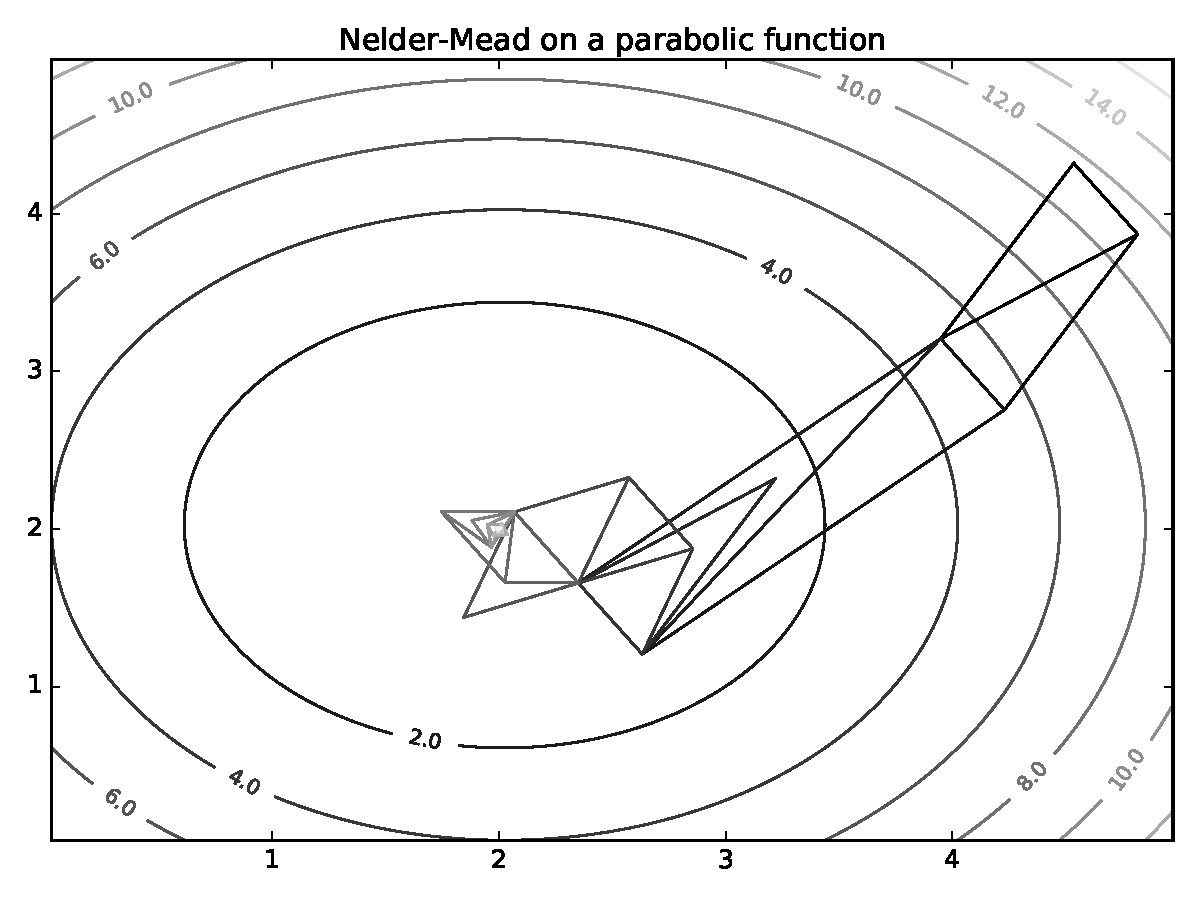
\includegraphics[width=8cm]{figs/neldermeadsimplex.pdf}}
\subfloat[Convergência do Nelder-Mead]{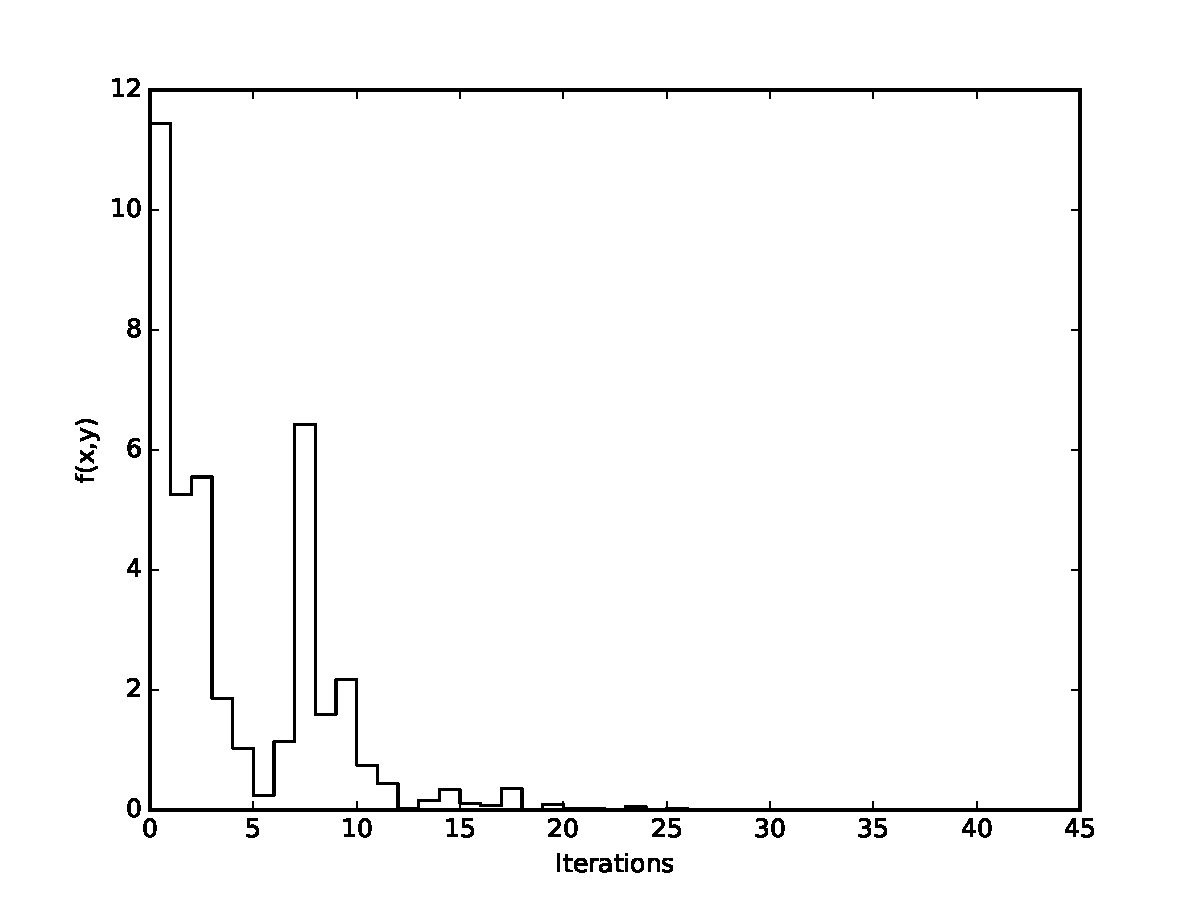
\includegraphics[width=8cm]{figs/neldermeadconvergence.pdf}}
\caption{Nelder-Mead aplicado em um parabolóide.}
\label{fig:neldermead}
\end{figure}



\begin{algorithm}
    \caption{Nelder-Mead's Downhill Simplex}
    \label{alg:int_point_ocp}
    \begin{algorithmic}[1] % The number tells where the line numbering should start
        \Require $X = (x_1, ... , x_{n+1})$ pontos de teste:
            \While{Não Convergiu}
                \State ordenar X; ($f(x _1) \leq f(({x} _2) \leq \cdots \leq f(x_{n+1})$) 
                \State Calcular o centroide $x_0$ de $(x_{1}, ... , x_{n+1})$
                \State Calcular $x_r$ refletido: $x_r = x_0 + \alpha(x_0 - x_{n+1})$ 
                
\BState \emph{(Reflecção)}                
                \If{  $f(f(x_1) < f(x_r) < f(x_n) $ }
                    \State $x_{n+1} \gets x_r$
                    \State Continue
                \EndIf

\BState \emph{(Expansão)}
                \If{  $f(f(x_r) < f(x_1)$ }
                    \State Calcular ponto expandido $x_e = x_0 + \gamma(x_r - x_0) $
                    \If{$f(x_e) < f(x_r)$}
                        \State $x_n \gets x_e$
                    \Else
                        \State $x_n \gets x_r$                  
                    \EndIf
                    \State Continue
                \EndIf
\BState \emph{(Contração)}
                \State Computar o ponto contraído $x_c = x_0 + \rho(x_{n+1} - x_0)$
                \If{$f(x_c) < f(x_{n+1})$}
                    \State $x_{n+1} \gets x_c$
                    \State Continue             
                \EndIf
\BState \emph{(Encolhimento)}
                \State $x_i \gets x_1 + \sigma(x_i - x_1), i=2 \dots n+1$
            \EndWhile
    \end{algorithmic}
\end{algorithm}



%%%%
%
\section{Baricenter Method}


%%%
%%
\section{OrthoMADS}

Os métodos MADS (Mesh Adaptative Direct Search) são uma classe de métodos baseados ...


A cada iteração $ k $ são executados dois passos de busca, Search e Poll, analisando a feasibility e valor da função. O objetivo de cada nova iteração é encontrar um ponto $f(x) < f(x_k)$, aonde $x_k$ é o melhor ponto encontrado até a iteração atual. 

As buscas são feitas sempre em uma grade, definida por:

$M_k = \{x + \Delta^m_kDz : x \in V_k, z \in \mathbb{N}^{nD} \} \subset \mathbb{R}^n$
Aonde $M_k$ é o conjunto de pontos da grade, $x$ é o ponto mínimo atual, $\Delta^m_k$ é o parametro de tamanho da malha, $D$ é uma matrix $\mathbb{R}^{n \times n_D}$ composta por $n_D$ direções que definem um conjunto gerador position no $\mathbb{R}^n$. Para o OrthoMads e LtMads, D é simplesmente definida como $[I_n -I_n]$ aonde $I_n$ é a matriz identidade de dimensões $n$.

O passo search pode ser qualquer tipo de heurística que escolha um ponto mais adequado da malha para tentar acelerar a convergência.

O passo poll é a parte mais importante do método, que garante sua convergência. A cada iteração $k$ os pontos a serem utilizados são definidos por:

\begin{center}
$P_k = \{ x_k + \Delta^p_kd : d \in D_k\} \subset M_k$
\end{center}

Aonde  $x_k$ é o ponto atual e cada coluna de $D_k$ é formada por combinações inteiras das colunas de $D$ de forma a criar um conjunto gerador positivo. $\Delta^p_k$ é o \textit{parametro de tamanho de poll}.

Ambos LtMads e OrthoMads utilizam um parametro $\ell_k$ chamado de \textit{indíce de malha} para atualizar os parametros de tamanho de poll e search de acordo com esta lógica:


\begin{equation} \label{eq:meshsizeupdate}
\Delta^p_k = 2^{-\ell k} \text{ e }  \Delta^m_k = min\{1, 4^{-\ell_k}\}
\end{equation}

A cada nova iteração, se em uma iteração um novo \textit{incumbente} não é encontrado, ela é dita mal sucedida, e $\ell_{k+1} \gets \ell_k +1$ (reduzindo $\Delta^m_k$ e $\Delta^p_k$), por outro lado, se for encontrado um novo \textit{incumbente}, a iteração é dita bem sucedidade, e $\ell_{k+1} \gets \ell_k -1$ (aumentando $\Delta^m_k$ e $\Delta^p_k$). Devido a \ref{eq:meshsizeupdate}, no caso de uma iteração mal-sucedida o parametro de poll diminui mais rápido que o de malha, de modo a permitir o uso de muitos mais pontos, refinando a malha.


A diferença entre o OrthoMads e LtMads se dá na geração da base $D_k$. O LtMads utiliza uma matriz triangular inferior para a geração da base, fazendo permutações entre os elementos e completando ela em uma base maximal ou minimal, sem garantir ortogonalidade entre as direções, de modo que os ângulos entre as direções podem ser grandes, causando grandes cones de espaço não explorado.
Já o OrthoMads utiliza uma base maximal definida por $[H_k -H_k]$, aonde as colunas de $H_k$ formam um base ortogonal de $\mathbb{R}^n$. Além disso, os as direções de $D_k$ são inteiras, de modo que os pontos gerados estão automaticamente contidos na malha definida por $D=[I_n -I_n]$.

Para a geração de $D_k$, o OrthoMads utiliza a sequencia pseudo-aleatoria de Halton, que cobre mais uniformemente o espaço que uma sequência aleatória real, para  gerar vetores $u_t$.

A saída da sequência de Halton, no entanto, não respeita as restrições impostas pela malha. É necessário arrondar, escalar, e rotacionar o vetor $u_t$. O indíce $\ell$ é utilizado para transformar a direção $u_t$ na \textit{direção ajustada de Halton} $q_{t,\ell} \in \mathbb{Z}^n$, uma direção cuja norma é próxima a a $2^{\frac{|\ell|}{2}}$

HERE, BLACK MAGIC IS USED TO MAKE THE VECTOR ALIGN TO THE MESH.

Para definir $q_{t,\ell}$, primeiramente são definidas duas funções baseadas na t-ésima direção de Halton $u_t$:

$q_t(\alpha) = \text{round} \left ( \alpha \cfrac{2u_t - e}{||2u_t - e||} \right ) \in \mathbb{Z}^n \cap \left [ -\alpha - \cfrac{1}{2}, \alpha + \cfrac{1}{2}  \right ]^n$

Aonde \textit{round} é a operação arrendodar para cima ($round(0,5)=1$, $round(-0,5) = -1$) e $\alpha \in \mathbb{R}_+$ é um fator de escala. 

Desta forma, temos um problema de otimização, precisamos encontrar um $\alpha_{t,\ell}$ tal que $||q_t(\alpha_{t,\ell})$ seja o mais próximo possível de $2^{\frac{|\ell|}{2}}$ sem ultrapassá-lo.

\begin{align*}
\alpha_{t,\ell} \in \underset{\alpha in \mathbb{R}_+}{\textit{argmax}} & ||q_t(\alpha)|| \\
\text{s.t.} & ||q_t(\alpha)|| \leq 2^{\frac{|\ell|}{2}}
\end{align*}

O problema pode ser resolvido facilmente, já que que os degraus da função $||q_t(\alpha)||$ acontecem em todos os $\alpha$ no conjunto

\begin{center}
$ \left \{ \cfrac{(2j+1)||2u_t - e||}{2|u^i_t - e|} : i = 1,2,\dots,n,j \in \mathbb{N} \right \}$
\end{center}
De forma que o problema pode ser solucionado varrendo os pontos do conjunto.

Com um vetor normalizado e na malha, $q \in \mathbb{Z}^n$, é necessário transformá-lo em uma base ortonormal de $\mathbb{R}^n$. Para isto é utilizada a transformação de Householder:

\begin{equation}
H = ||q^2||(I_n - 2vv^T),\textit{ onde }v = \cfrac{q}{||q||}
\end{equation}

Aonde $H$ é uma base ortonormal gerada a partir de $q$.

Com a base ortonormal criada, podemos utilizar o algoritmo~\ref{alg:orthomads}, comum ao LtMads e OrthoMads.

ALGO MAIS DEVE SER ESCRITO AQUI, MAS OQ?


\begin{algorithm}
    \caption{OrthoMads}
    \label{alg:orthomads}
    \begin{algorithmic}[1] % The number tells where the line numbering should start
\BState \emph{[0] Inicialização}   
                \State $x_0 \in \Omega , \ell_0 \gets 0, k \gets 0, t_0 \gets p_n$ 
            \While{Não Convergiu}
\BState \emph{(ITERAÇÃO $k$)}                
            \State Search (opcional)
			\State Avalia $ f $ em um conjunto finito $S_k \subset M_k $
\State \emph{POLL}
    \If{o tamanho do parametro POLL é o menor até então ($ \Delta^p_k = \text{min} \{ \Delta^p_j : j=  0,1,\dots,k \}$)} 
    \State $t_k \gets \ell_k + t_0$
    \Else{ (Já foram considerados tamanhos menores)}
    \State $t_k \gets 1 + \text{max} \{t_j:j=0,1,\dots,k-1\}$
    \EndIf
    \State Computa $ u_{tk} , q_{tk}   \ell_k $ and $ D_k = \big[ H_{tk} \text{    } -H_{tk} \big] $
\BState \emph{UPDATES}                
	\If{ A iteração foi bem sucedida ( se existe um $x_s \in S_k \text{ ou } x_p \in P_k$ tal que $f(x_s) < f(x_k)$ ou $ f(x_p) < f(x_k)$ }
		\State $x_{k+1} \gets x_s $ or $x_p$
		\State $\ell_{k+1} \gets \ell_k - 1$
	\Else {(iteração falhou)}
		\State $x_{k+1} \gets x_k$
		\State $\ell_{k+1} \gets \ell_k + 1$
    \EndIf
    \State $k \gets k + 1$
    \EndWhile
    \end{algorithmic}
\end{algorithm}



%%%%%%%%%%%%%%%%%


\chapter{Ferramentas Computacionais} \label{chap:4}


\section{O Simulador Pipesim}
Sistemas de produção de petróleo são sistemas nos quais se deseja sempre produzir o máximo possível e de forma segura.
O PIPESIM, da Schlumberger, é um simulador de fluxo multifásico em regime permanente que pode ser utilizado tanto para o projeto como para planejamento de operações em campos de petróleo. Ele permite que sejam simuladas situações alternativas de forma mais rápida e segura que testes reais. É possível simular desde um único poço, como no projeto atual, até uma complexa rede de produção como as em uso pela Petrobras.

\section{Python}

O Python é uma linguagem de alto nível, interpretada, de desenvolvimento rápido muito utilizada para prototipação e na academia. Suas faciliades, como Jupyter Notebook \cite{jupyter}, um ambiente que facilita a criação de documentos com códigos e análise de dados, e o Matplotlib \cite{matplotlib}, uma biblioteca que a torna quase tão poderosa quando o MatLab para visualização de dados, a tornaram muito utilizada também na academia.

Python tem como filosofia de design a legibilidade do código (foi escolhido o uso de espaços no lugar de chaves pra delimitação de blocos de código) e uma linguagem que facilita a expressão de conceitos complexos em poucas linhas de código se comparada, por exemplo, com Java ou C++. A linguagem expõe estruturas e conceitos complexos em outras linguagens de forma mais fácil e intuitiva de utilizar.

A Linguagem surgiu em 1991 \cite{pythonHistory}, e segundo Tiobe \cite{tiobe} é a quarta linguagem de programação mais popular atualmente.

Sua facilidade de uso, expêriencia prévia não necessária, disponibilidade de ferramentas, e facilidades de visualização de dados foram decisivos para a sua escolha para este trabalho. 

\section{Interface Python e Open Link}
Para interfaceamento do Pipesim com outros software, a Schlumberger disponibiliza uma API (Application Programming Interface) chamada Open Link, idealizada para programação em C++, VBA, ou Visual Basic. Esta pode ser utilizada para interação programática com o Pipesim, habilitando a configuração de novos poços, alteração de poços existentes, análises, simulações e automação de simulações. Com essa API, é possível variar os parâmetros do poço e avaliar as curvas características.




 Utilizando-se a biblioteca de Python pyWin32, é possível comunicar-se com a API, mas apenas em versões do Windows de 32 bits. Apesar de algumas peculiaridades no tratamento de arrays e outros tipos de dados, esta biblioteca permite o uso da API em uma linguagem de desenvolvimento mais rápido\cite{pythonfast} e com grandes facilidades de análise de dados.

\section{NOMAD}
Para utilização do orthoMADS, foi escolhida a ferramenta NOMAD \cite{Nomad}, uma implementação em C++ do orthoMADS desenvolvida pelo GERAD \cite{gerad}, um centro de pesquisa multi-universidades canadenses.
%
Seu objetivo é a solução de problemas de otimização sem-derivadas com problemas caixa-preta, aonde não se conhece o modelo explícito do problema.
%
Bastando fornecer uma função objetivo e restrições, a ferramenta é capaz de encontrar um ponto ótimo para o problema.
 %
Ela também disponibiliza variações do algoritmo (como $2n$ ou $n+1$ bases) e a possibilidade de paralelismo (consultar mais que um ponto de forma concorrente).  

	

\section{Opal}
Para o uso do NOMAD com o Python, era sugerido, até o começo destes trabalhos, o uso da ferramenta Opal \cite{opal} (A Framework for Optimization of Algorithms). Uma interface open-source de alto nível para a interface de Python com o NOMAD. Este framework dá a liberdade para configurar todos os parâmetros de otimização do NOMAD e também é capaz de paralelismo.

No entanto ele suporta apenas Python 2.7 que está para ser aposentado em 2020 \cite{python27sched}, de modo que foi necessário portá-lo para Python 3 \cite{opalPython3}, contribuição que deve ser enviada para os repositórios originais assim que finalizada.

É interessante ressaltar também que a partir da versão 3.8.0 do NOMAD, foi implementada um interface própria em Python (novamente Python2.7) que deve ser analisada para uso em trabalhos futuros.

O Opal é um framework complexo, que embora seja utilizado atualmente apenas para o uso do NOMAD, contém a base para implementação de outros solvers genéricos, suporte a paralelismo, e a outras plataformas, como Sun Grid Engine e Symmetric Multiproccessing (SMP).


%%%%%%%%%%%%%%%


\chapter{O Problema de Sintonia} \label{chap:conc}
	

A sintonia de simuladores de poços de petróleo costuma ser feita a partir de dados experimentais. 
%
A partir de testes de campo, adquirem-se pontos de testes do sistema real.
%
Os pontos reais são utilizados como referência para que o operador varie os parâmetros de forma a encontrar o modelo que melhor represente os dados coletados.
%

Para os testes neste trabalho, primeiramente foi configurado um único poço de petróleo, com uma estrutura simples e que pode ser visto na figura \ref{fig:setup1_dia}.
% 
A seguir foram escolhidos dados arbitrariamente para compor a curva ``real'' de produção (figura \ref{fig:truth1}).
%
Neste Experimento a curva sintonizada foi a de fluxo de líquido (Barris padrões por dia) por gás injetado (milhões de pés cúbicos padrões por dia), no entanto é possível utilizar outras curvas, ou ainda mais que uma, para a sintonia.
%

Escolheu-se a pressão estática do reservatório como sendo 4000 psi absoluto, e um índice de produtividade de líquido de 25 STDB/d/psi (barris padrões por dia por pressão estática). 
%
Desta forma a figura \ref{fig:truth1} demonstra o poço ``real'' a ser sintonizado.



\begin{figure}[H]
\centering
\begin{subfigure}{.25\textwidth}
  \centering
  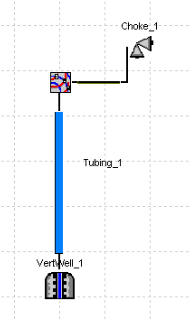
\includegraphics[width=1\linewidth]{figs/setup1.png}
  \caption{Setup do poço de petróleo.}
  \label{fig:setup1_dia}
\end{subfigure}%
\begin{subfigure}{.75\textwidth}
  \centering
  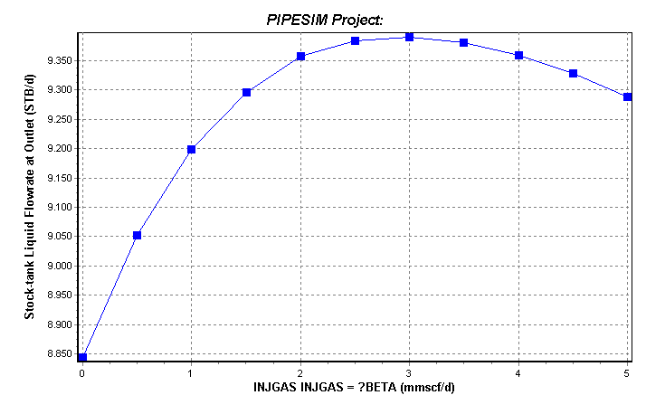
\includegraphics[width=1\linewidth]{figs/truth1.png}
  \caption{Curva ``real'' do poço de petróleo.}
  \label{fig:truth1}
\end{subfigure}
\caption{Configuração e curva do poço do experimento 1.}
\label{fig:setup1}
\end{figure}

Em todos os testes, os parâmetros $s_p$ (pressão estática) e $l_{pi}$ (Índice de produção de líquido) foram iniciados respectivamente em 3000 (psi) e 15 (STDB/d). A interface OpenLink foi utilizada para modificar os parâmetros e ler uma nova curva de fluxo de líquido por injeção de gás, a distância quadrática entre as duas curvas foi utilizada como o erro na otimização.

O problema de otimização, então, é dado por 
\begin{align}
\min\limits_{x \in \Omega} f(x)
\end{align}
Onde
\begin{align}
x = &(s_p, l_{pi})\\
\Omega = &\{s_p \in \mathbb{R} \mid s_{p,min} < s_p < s_{p,max}\}\\
          &\{l_{pi} \in \mathbb{R} \mid  l_{pi,min} < l_{pi} < l_{pi,max}\}
\end{align}
Onde $s_p$ é a pressão estática do reservatório e $l_{pi}$ é o índice de produtividade de líquidos. 

Seja $f(q_{inj};x)$ a produção de líquido estimada pelo simulador quando sintonizado com parâmetros $x$ ao se injetar $q_{inj}$ gás no poço, e seja $\theta(q_{inj};x)$ a produção ``real'' de líquido com parâmetros $x$.
\begin{align}
f(x) &= f(s_p, l_{pi}) \\
     &= \sum_{i=1}^n \Big[ \theta(q_{inj}^n;x) - f(q_{inj}^n;x))\Big]^2
\end{align}
Onde $q_{inj}^1, q_{inj}^2, \dots, q_{inj}^n$ são os pontos amostrados da curva de produção. 

Neste problemas foram impostos: 
\begin{align*}
l_{pi,min}&= 15\\
l_{pi,max}&= 35\\
s_{p,min} &= 2000\\
s_{p,max} &= 7000\\
\end{align*}
\chapter{O Experimento de Sintonia Sem Ruído}

Foram realizados três experimentos de sintonia de curva, e utilizadas três abordagens diferentes para a sintonia. Primeiramente foi utilizado o OrthoMADS, com a implementação NOMAD, em seguida, foi utilizado novamente o NOMAD, mas com um surrogate model calculado pela SGTELIB, e finalmente, uma implementação do Nelder-Mead Simplex. Os resultados então são comparados quanto a número de avaliações e acurácia do resultado.

Os experimentos foram realizados em uma máquina virtual VirtualBox, rodando em um Xeon 2665, e utilizando dois núcleos.

\section{Setup para sintonia de curva com o orthoMADS}
Para a sintonia com o orthoMADS, foi utilizado o framework OPAL (A Framework for Optimization of Algorithms), interface Python para o solver NOMAD.
A implementação com o OPAL utiliza dois arquivos, "well\_declaration.py" e "well\_optimize.py".

O arquivo "well\_declaration.py" expõe os componentes do problema:

\begin{itemize}
\item Nome do algoritmo:
\begin{lstlisting}[language=Python]
# Define Algorithm object.
tuning = Algorithm(name='TUNING', description='Well Tuning')
\end{lstlisting}
\end{itemize}

\begin{itemize}
\item Comando utilizado pelo solver para avaliar a função:
\begin{lstlisting}[language=Python]
tuning.set_executable_command('python pipesim_run.py')
\end{lstlisting}
\end{itemize}


\begin{itemize}
\item As variáveis de decisão:
\begin{lstlisting}[language=Python]
static_pressure = Parameter(kind='real', 
                            default=sp, 
                            bound=(2000, 7000),
                            name='sp', 
                            description='Static Pressure')
liq_pi = Parameter(kind='real', 
                   default=pi, 
                   bound=(15, 35),
                   name='pi', 
                   description='Liq PI')

FD.add_param(static_pressure)
FD.add_param(liq_pi)
\end{lstlisting}
\end{itemize}

\begin{itemize}
\item E o erro:
\begin{lstlisting}[language=Python]
error = Measure(kind='real', name='ERROR', description='Curve quadratic error')
FD.add_measure(error)
\end{lstlisting}
\end{itemize}

Já no arquivo "well\_optimize", são declaradas estruturas auxiliares:
\begin{itemize}

\item É instanciado o solver:
\begin{lstlisting}[language=Python]%

def get_error(parameters, measures):
    return sum(measures["ERROR"])

data = ModelData(FD)
struct = ModelStructure(objective=get_error)  # Unconstrained
model = Model(modelData=data, modelStructure=struct)

NOMAD = NOMADSolver()

\end{lstlisting}



\item São impostas as seguintes restrições ao solver do NOMAD:
\begin{lstlisting}[language=Python]
F_TARGET = 0.1
\end{lstlisting}

De modo a limitar o tamanho mínimo da malha, e terminar a simulação quando a função custo chegar a um valor abaixo de 0.1

\item E é inicilizada a otimização:
\begin{lstlisting}[language=Python]
NOMAD.solve(blackbox=model)
\end{lstlisting}

\end{itemize}

\section{Resultados da Sintonia de Curva com o orthoMADS}

Em 525 segundos (8:45 minutos) e com de 206 avaliações de caixa preta. A performance do algoritmo pode ser vista na figura \ref{fig:setup1_2}. A parada se deu pelo valor da função custo estar abaixo de 0,1. A convergência se deu para os seguintes valores:

\begin{align*}
s_p&= 4000,691 \\
l_{pi} &= 24,954 \\
Custo &= 0,0757.
\end{align*}

Que são muito próximos aos valores reais $s_p=4000$ e $l_{pi}=25$.


\begin{figure}[H]
\centering
\begin{subfigure}{0.5\textwidth}
  \centering
  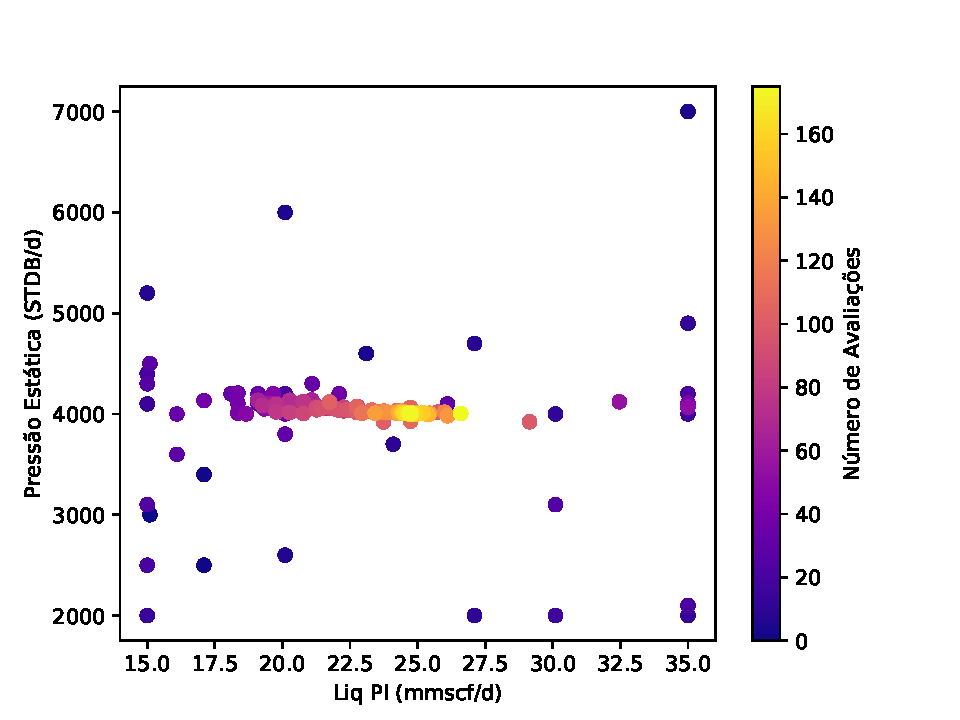
\includegraphics[width=1\linewidth]{figs/setup1_eval_points.pdf}
  \caption{Pontos escolhidos pelo NOMAD.}
  \label{fig:setup1_points}
\end{subfigure}%
\begin{subfigure}{0.5\textwidth}
  \centering
  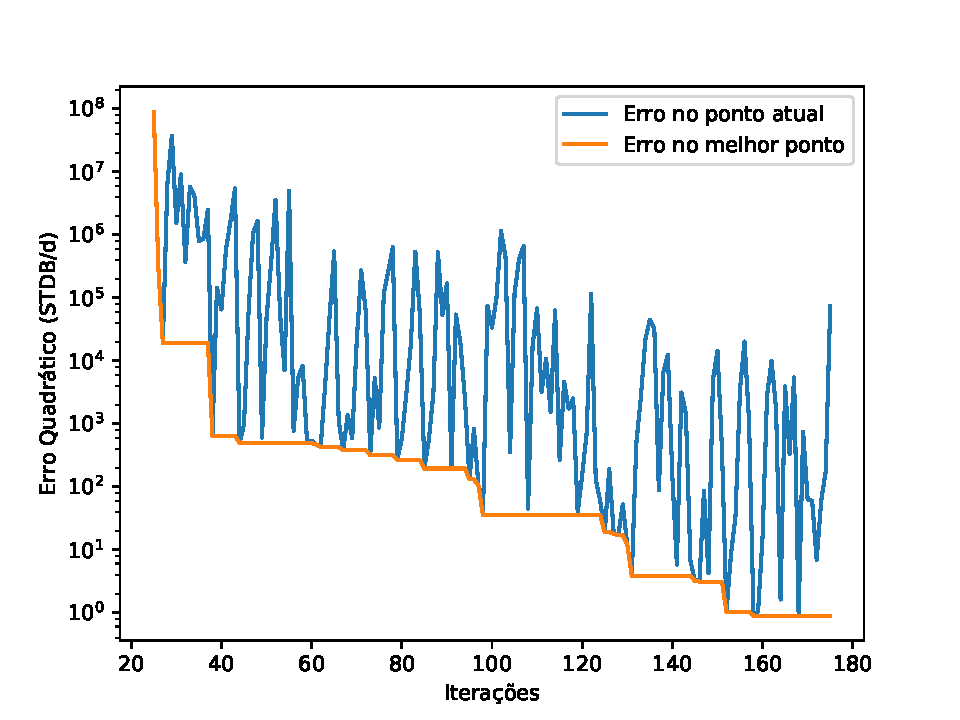
\includegraphics[width=1\linewidth]{figs/setup1_errors.pdf}
  \caption{Erro nos pontos avaliados.}
  \label{fig:setup1_error}
\end{subfigure}
\caption{NOMAD aplicado ao experimento 1.}
\label{fig:setup1_2}
\end{figure}

\section{A Surrogate Lib}

Durante a realização desses experimentos, o NOMAD foi atualizado e recebeu uma ferramenta auxiliar, uma biblioteca que tenta aproximar a função a partir dos pontos já utilizados, para utilização no passo "search" do algoritmo. Esta biblioteca faz com que o algoritmo, a cada iteração, tente adivinhar a melhor direção para avançar, ao invés de progredir aleatoriamente.

Para o cálculo do modelo substituto, são possíveis nove tipos de modelos, que podem ser vistos na documentação, além de onze tipos possíveis de núcleos. Neste trabalho foram utilizadas as opções padrão do NOMAD, um modelo PRS (Polynomial Response Surface) de ordem 2.


\section{Setup Para Sintonia de Curva Com a Surrogate Lib}

Um contra-tempo quanto a SGTELIB, como é chamada a biblioteca, é que ela está embutida nos binários do NOMAD, e, por algum erro, os binários para windows foram compilados com uma versão antiga do Microsoft Visual Studio, de forma que é necessário recompilar não apenas o SGTELIB (o que pode ser feito com o mingW sem grandes mudanças), mas todo o NOMAD, necessitando a instalação de aproximadamente 4Gb do Visual Studio.

Após sua recompilação, bastou substituir o binário antigo pelo novo, é inserir nos parâmetros do NOMAD para o uso da SGTELIB, com seus valores padrõess:
\begin{lstlisting}[language=Python]
NOMAD.set_parameter(name="MODEL_SEARCH", value="SGTELIB")
\end{lstlisting}
Para que ele passasse a utilizar o SGTELIB no local do seu SEARCH baseado em modelo quadrático.


\section{Resultados da Otimização Com a Surrogate Lib}

A execução demorou 1374 segundos (22:27 minutos) e necessitou de 417 avaliações de função de caixa preta. O Nomad novamente convergiu, desta vez para os 	valores:

\begin{align*}
s_p&= 4001,389 \\
L_{pi} &= 24,905 \\
Custo &= 0,09986.
\end{align*}
É possível notar, no entanto, que com o SGTELIB, em muitos pontos o erro quadrático saturou em $10^{64}$. Nota-se também que pontos longe do ótimo foram avaliados perto da convergência (pontos claros no canto inferior esquerdo), o que pode significar que existe um problema com a SGTELIB, ou que o modelo utilizado não é o ideal, talvez pelo fato de que as superfícies polinomiais tendam a crescer muito para longe na origem, levando o algoritmo a testar pontos distantes.

\begin{figure}
\centering
\begin{subfigure}{0.5\textwidth}
  \centering
  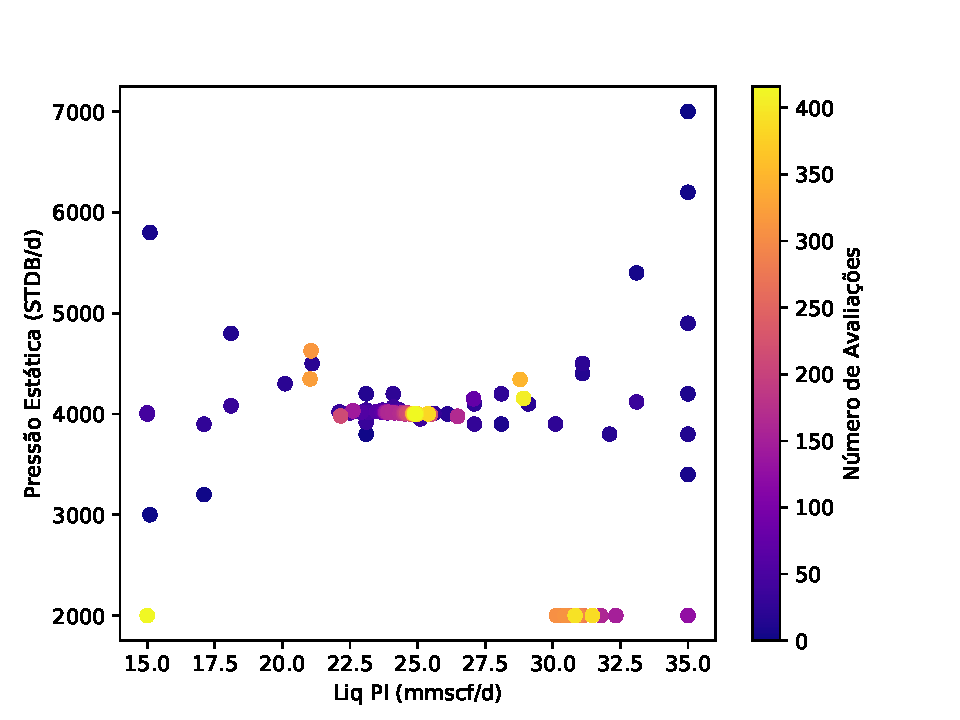
\includegraphics[width=1\linewidth]{figs/setup1sgtelib_eval_points.pdf}
  \caption{Pontos escolhidos pelo NOMAD.}
  \label{fig:setup2_points}
\end{subfigure}%
\begin{subfigure}{0.5\textwidth}
  \centering
  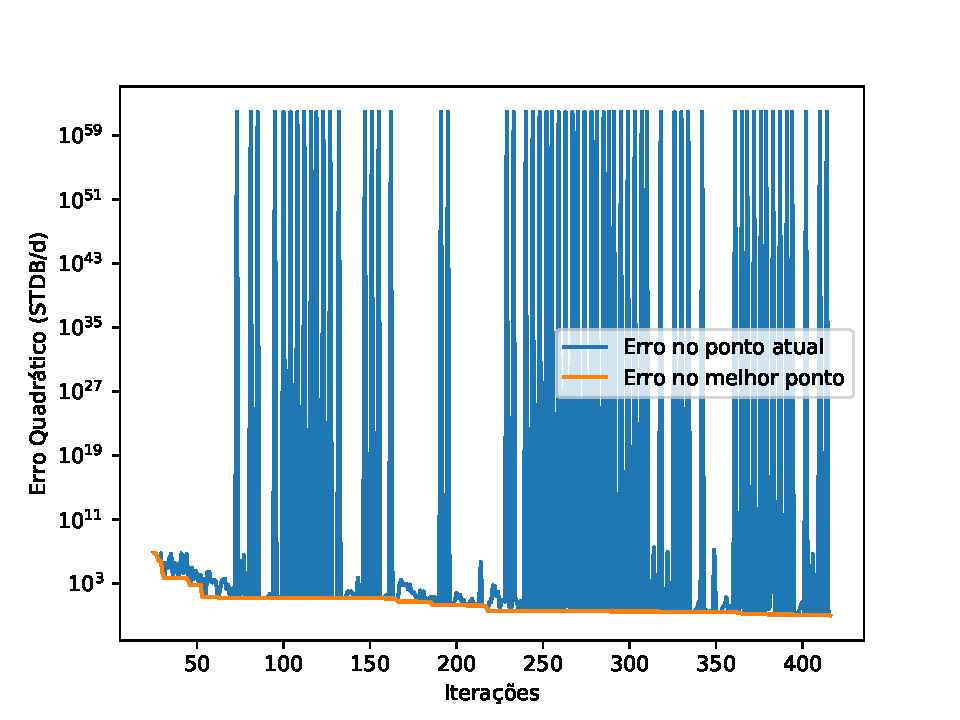
\includegraphics[width=1\linewidth]{figs/setup1sgtelib_errors.pdf}
  \caption{Erro nos pontos avaliados.}
  \label{fig:setup2_error}
\end{subfigure}
\caption{NOMAD aplicado ao experimento 1 com SGTELIB.}
\label{fig:setup2_2}
\end{figure}


\section{Setup da Otimização com Nelder-Mead Simplex}

Para o teste com o Simplex de Nelder-Mead, foi utilizada uma implementação própria, baseada no algoritmo \ref{alg:nm}, e como ele não é facilmente paralelizável, não houveram preocupações com paralelismo.
Os limites utilizados foram os mesmos dos casos anteriores:
\begin{align}
15 < &l_{pi} < 35 \\
2000 < &s_p < 7000
\end{align}

Como o simplex utiliza uma estrutura $n$-dimensional para a busca, são necessários $n+1$ pontos iniciais, por este motivo um triângulo foi expandido arbitrariamente a partir do ponto inicial, de modo que no começo do algoritmo, o simplex inicial seja grande. As restrições foram aplicadas somando-se um peso adicional a função custo.

Os resultados podem ser vistos nas figuras \ref{fig:setup3_2} e \ref{fig:setup3_triang}. Nota-se que a solução foi mais rápida, com 212 iterações em 133 segundos (2:13 minutos). No entanto, o método de Nelder e Mead não tem as mesmas características de convergência que os os métodos MADS. É interessante comentar o caso da figura 5, aonde é possível notar que o simplex primeiramente moveu-se para um ponto em torno de $l_{pi}=18$, depois moveu-se lentamente para o ponto final:

\begin{align*}
s_p&= 4001,389 \\
l_{pi} &= 24,905 \\
Custo &= 0,09986.
\end{align*}


\begin{figure}
\centering
\begin{subfigure}{0.5\textwidth}
  \centering
  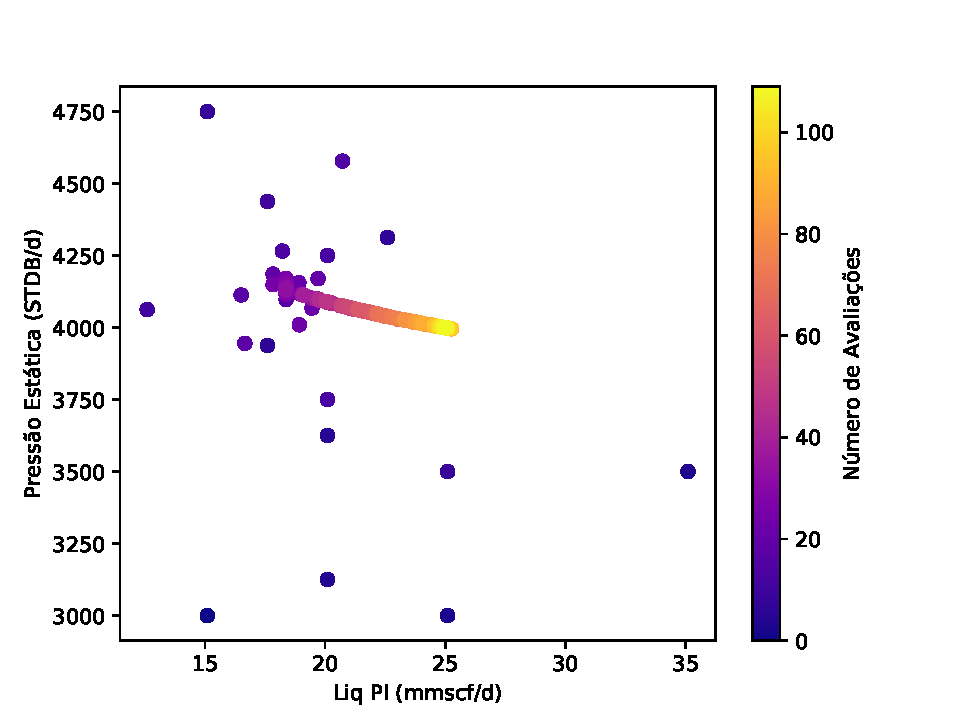
\includegraphics[width=1\linewidth]{figs/setup1nm_eval_points.pdf}
  \caption{Pontos escolhidos pelo Nelder-Mead.}
  \label{fig:setup3_points}
\end{subfigure}%
\begin{subfigure}{0.5\textwidth}
  \centering
  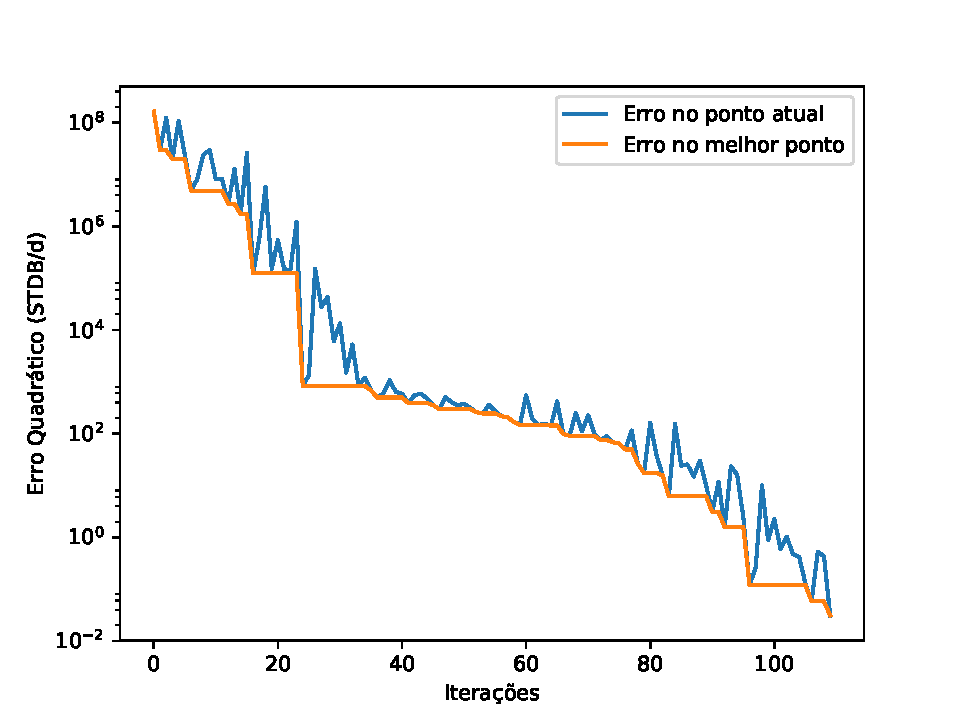
\includegraphics[width=1\linewidth]{figs/setup1nm_errors.pdf}
  \caption{Erro nos pontos avaliados.}
  \label{fig:setup3_error}
\end{subfigure}
\caption{Nelder-Mead aplicado ao experimento 1.}
\label{fig:setup3_2}
\end{figure}

\begin{figure}
\centering
	  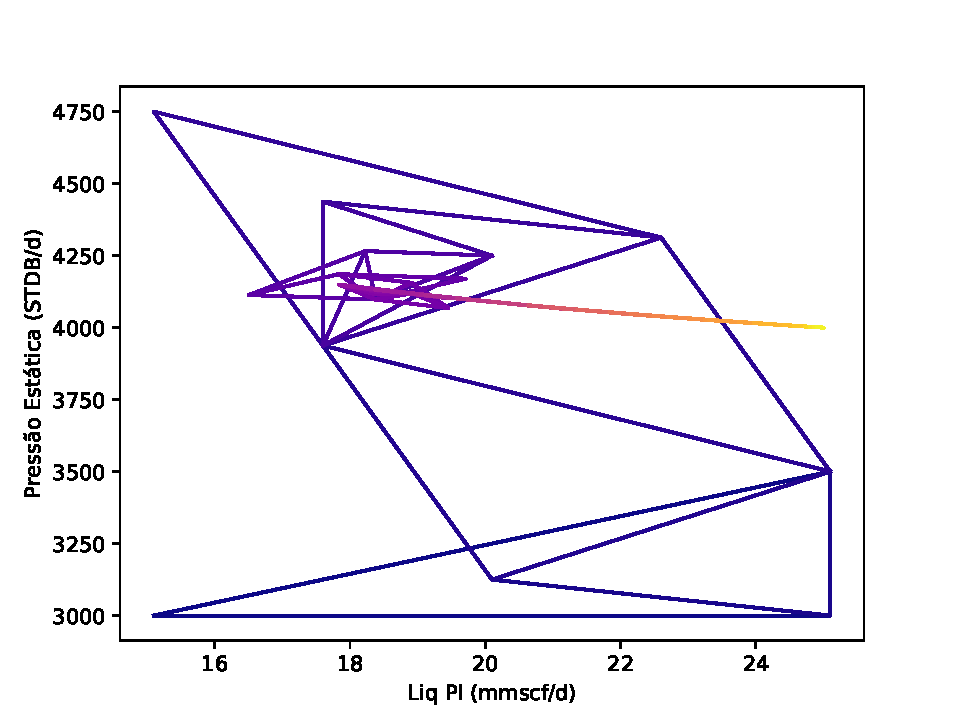
\includegraphics[width=0.7\linewidth]{figs/triangles_neldermead.pdf}
  \caption{Simplexes utilizados pelo Nelder-Mead.}
  \label{fig:setup3_triang}
\end{figure}




\section{Discussão}

É possível notar, pela figura \ref{fig:comp1} e pela \ref{tab:res1} que o Nelder-Mead, embora tenha utilizado um número semelhante de iterações que o orthoMADS, foi aproximadamente quatro vezes mais rápido. É possível que isso se dê pelo fato de que o OPAL, embora utilize várias \textit{threads}, talvez não faça um gerenciamento ideal do processador, e sim faça um \textit{busy wait}, que é quando um processo espera um sinal (no caso o fim de uma \textit{thread}) sem liberar o processador para outras \textit{threads}. Embora exista a suspeita do problema, não foi possível localizá-lo no código fonte.

Outra possível interpretação é que a diferença seja devido ao \textit{overhead} no NOMAD. Todas suas iterações envolvem o disparo de novos processos do Python, que por sua vez disparam o processo do Pipesim, além da escrita e leitura de diferentes arquivos para a comunicação entre os processos. Como a implementação utilizada do Nelder-Mead foi feita diretamente em Python, o \textit{overhead} existente é apenas a interface com Open Link.


\begin{table}[		]
\centering
\caption{Tempo de execução e numero de iterações por algoritmo}
\label{tab:res1}
\begin{tabular}{|l|l|l|}
\hline
                    & Tempo & Iterações \\ \hline
OrthoMADS           & 525   & 206       \\ \hline
OrthoMADS + SGTELIB & 1374  & 417       \\ \hline
Nelder-Mead         & 133   & 110        \\ \hline
\end{tabular}
\end{table}


\begin{figure}
\centering
  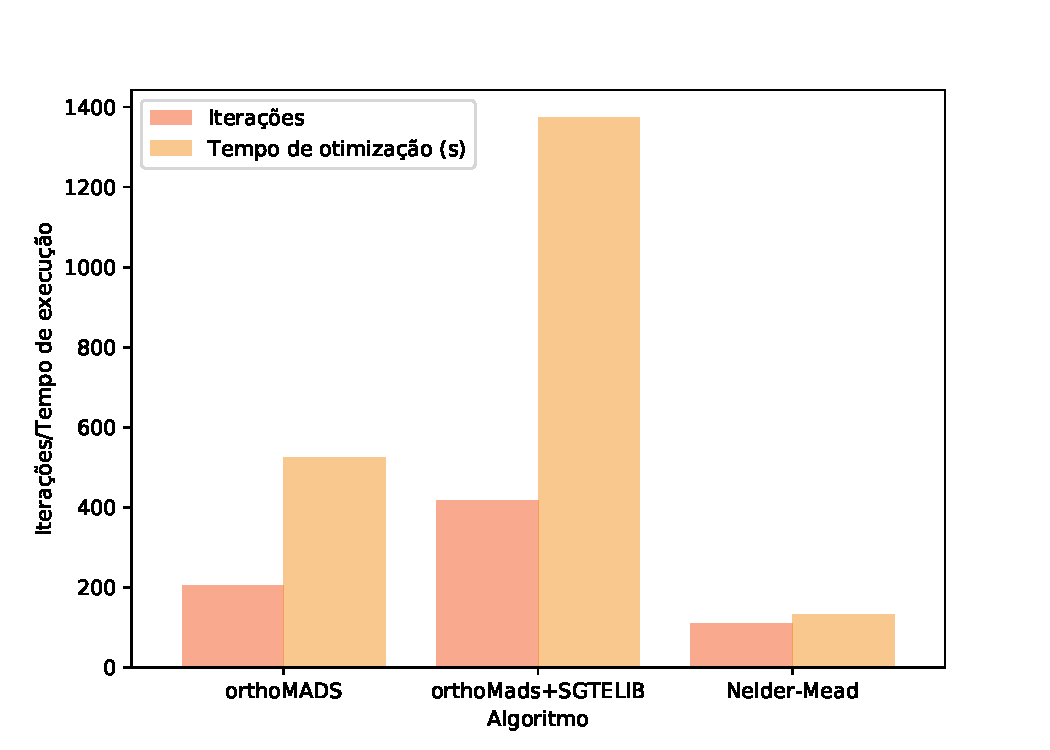
\includegraphics[width=0.7\linewidth]{figs/comp_time_iter.pdf}
  \caption{Comparação entre tempos de execução e número de iterações entre os três experimentos.}
  \label{fig:comp1}
\end{figure}


\chapter{O Experimento de Sintonia Com Ruído}

Para testar um caso um pouco mais realista, foram introduzidos ruídos ao sistema.
%
Primeiramente foi introduzido um ruído de medição nos pontos ``reais'' com desvio padrão $\sigma = 10$ (STDB/d) e média nula, para uma distribuição gaussiana.
%
Este ruído simula as condições adversas da medição em campo, perdas em sensores, sinais elétricos, imprecisões de montagem, e etc...
%
%

Adicionalmente, foi adicionado um pequeno ruído na simulação, para emular erros de precisão no caso de simuladores com soluções iterativas, que podem parar a simulação antes da precisão completa. 
%
A este ruído foi atribuído também uma distribuição normal com média zero, mas $\sigma = 10^{-5}$ para cada variável.
%
Como não existe mais a possibilidade um \textit{match} perfeito (zerar a função custo), é bom pensar no critério de parada. 
%
Como um balanço de precisão e execução, é escolhido o critério de que os pontos explorados estão a menos de $10^{-3}$ unidades de distância em cada variável.
%
Para as novas configurações, foram repetidos os experimentos.



\section{Sintonia de Curva com Ruído Com OrthoMADS}

Com o OrthoMADS, a otimização levou 334 segundos (5:34 minutos) e precisou de 130 avaliações. OS resultados podem ser analisados na figura \ref{fig:exp2_om}, que mostra os pontos avaliados e progressão do erro com as avaliações, e na figura \ref{fig:exp2_om_curve}, aonde é possível notar que a curva identificada está muito próxima a real, apesar do ruído na curva medida. 




\begin{figure}
\centering
\begin{subfigure}{0.5\textwidth}
  \centering
  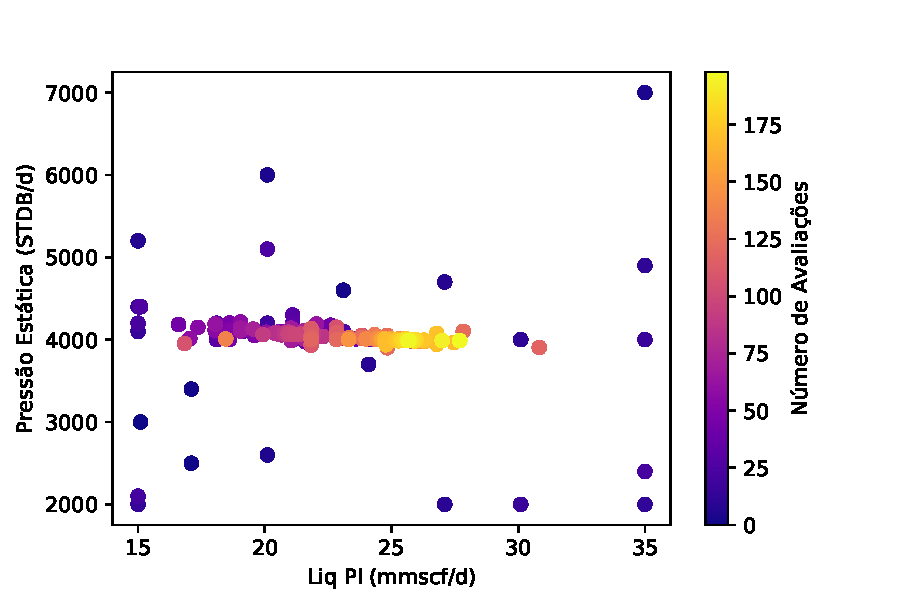
\includegraphics[width=1\linewidth]{figs/setup2_om_points.pdf}
  \caption{Pontos escolhidos pelo NOMAD.}
  \label{fig:exp2_om_points}
\end{subfigure}%
\begin{subfigure}{0.5\textwidth}
  \centering
  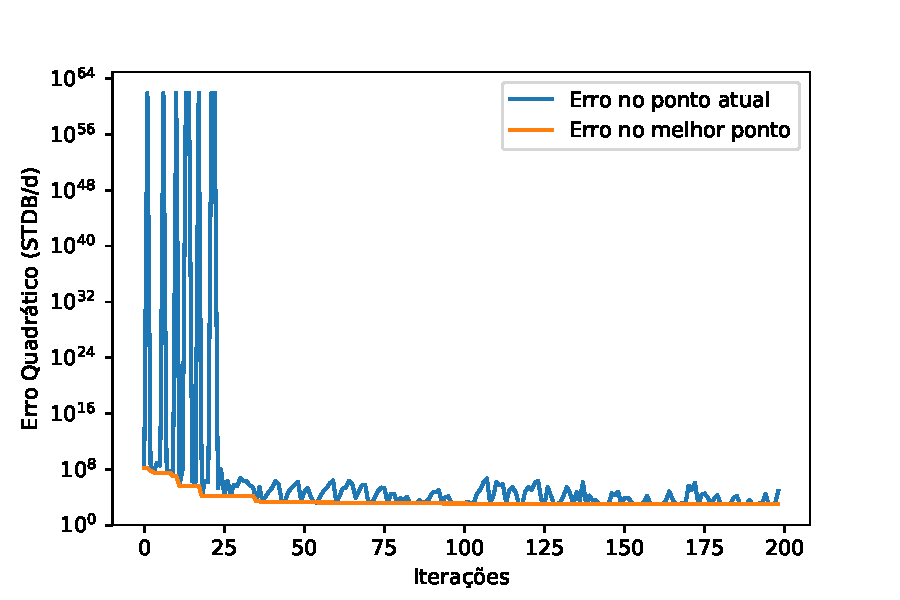
\includegraphics[width=1\linewidth]{figs/setup2_om_errors.pdf}
  \caption{Erro nos pontos avaliados.}
  \label{fig:exp2_om_error}
\end{subfigure}
\caption{NOMAD aplicado ao experimento 2.}
\label{fig:exp2_om}
\end{figure}





\begin{figure}
\centering
  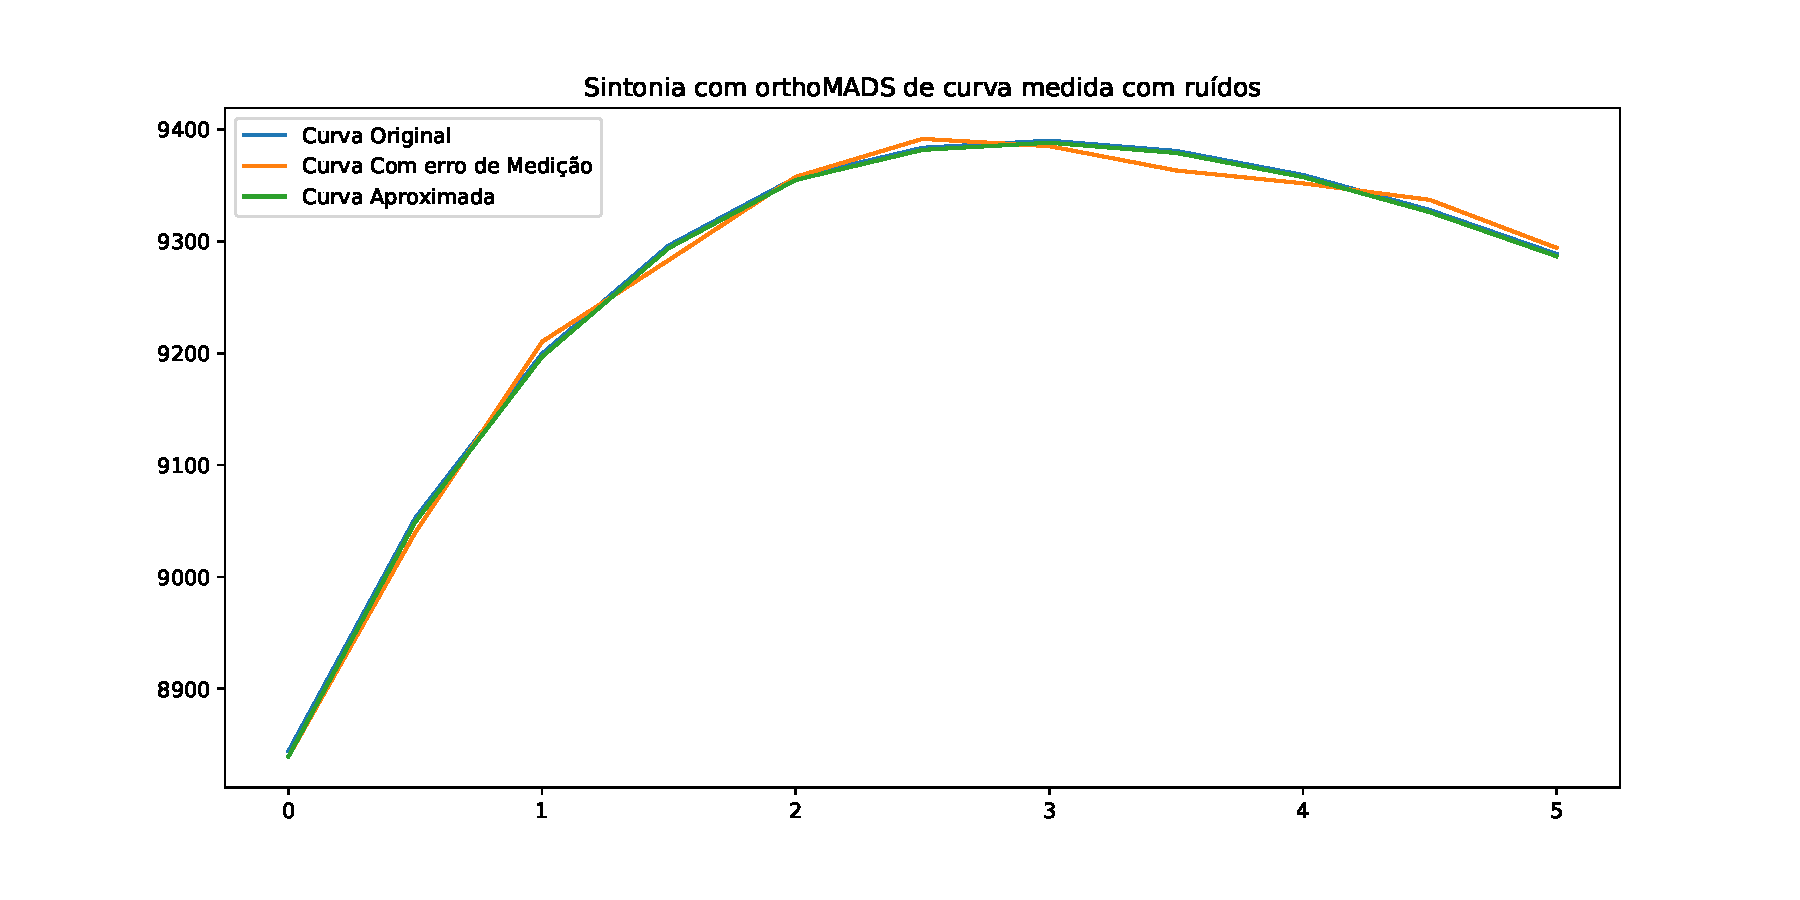
\includegraphics[width=1\linewidth]{figs/curva_om.pdf}
  \caption{Resultado da sintonia utilizando-se o OrthoMADS.}
  \label{fig:exp2_om_curve}
\end{figure}




\section{Sintonia de Curva com Ruído Com OrthoMADS + SGTELIB}

Com o OrthoMADS e a SGTELIB, a otimização levou 187 segundos (3:07 minutos) e precisou de 68 avaliações de caixa preta. Os resultados podem ser avaliados na figura \ref{fig:exp2_sg}, que mostra os pontos avaliados e progressão do erro com as avaliações, e na figura \ref{fig:exp2_sg_curve}, aonde é possível notar que a curva identificada também está muito próxima a real, apesar do ruído na curva medida. 
%

Também é notável que o novo método de SEARCH foi capaz de diminuir o número de avaliações (52\%).
%
Ele converge para um ponto próximo ao do método anterior (respectivamente 982,524 e 956,827), consumindo menos tempo e avaliações.


\begin{figure}[H]
\centering
\begin{subfigure}{0.5\textwidth}
  \centering
  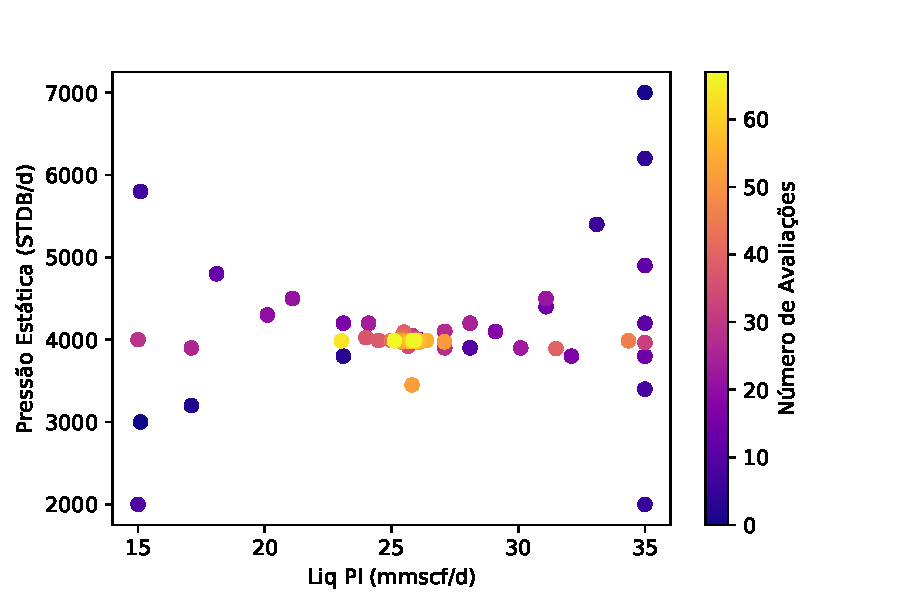
\includegraphics[width=1\linewidth]{figs/setup2_sg_points.pdf}
  \caption{Pontos escolhidos pelo NOMAD.}
  \label{fig:exp2_sg_points}
\end{subfigure}%
\begin{subfigure}{0.5\textwidth}
  \centering
  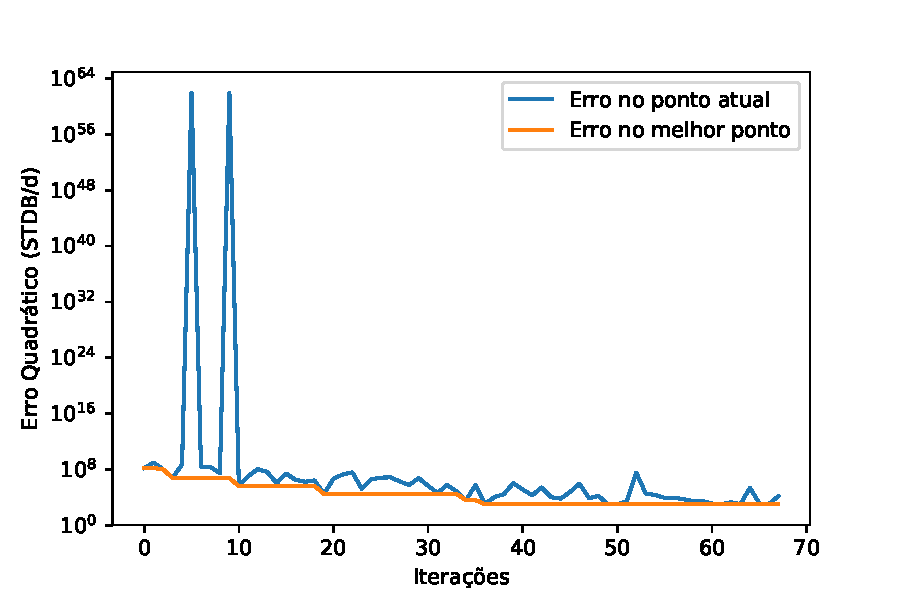
\includegraphics[width=1\linewidth]{figs/setup2noisy_sg_errors.pdf}
  \caption{Erro nos pontos avaliados.}
  \label{fig:exp2_sg_error}
\end{subfigure}
\caption{NOMAD com SGTELIB aplicado ao experimento 2.}
\label{fig:exp2_sg}
\end{figure}





\begin{figure}[H]
\centering
  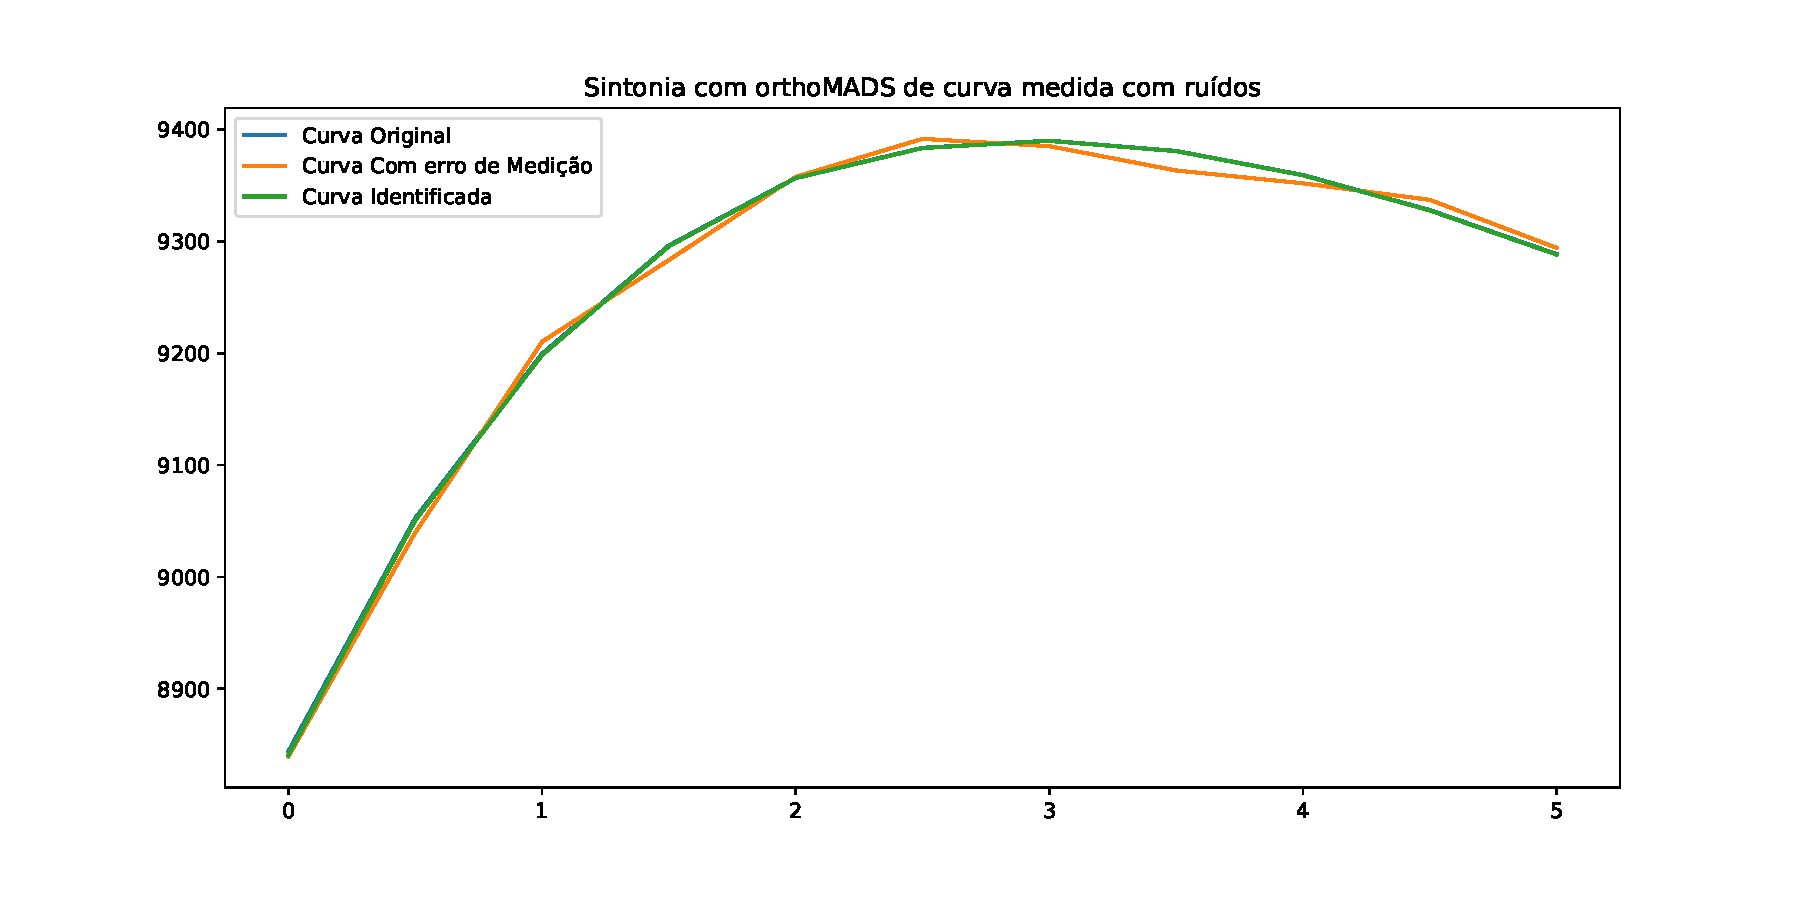
\includegraphics[width=1\linewidth]{figs/curva_sg.pdf}
  \caption{Resultado da sintonia utilizando-se o OrthoMADS com a SGTELIB.}
  \label{fig:exp2_sg_curve}
\end{figure}


\section{Sintonia de Curva com Ruído Com Nelder-Mead}

Com a utilização do algoritmo de Nelder-Mead, em 217 segundos (3:27 minutos) e 92 avaliações, o algoritmo convergiu com uma uma função custo em 953.623. Como pode se ver na figura \ref{fig:exp2_nm_error}, o algoritmo converge rapidamente no inicial, mas demora a adquirir a precisão requerida para a parada. Novamente a curva identificada está muito próxima da original sem ruídos.



\begin{figure}[H]
\centering
\begin{subfigure}{0.5\textwidth}
  \centering
  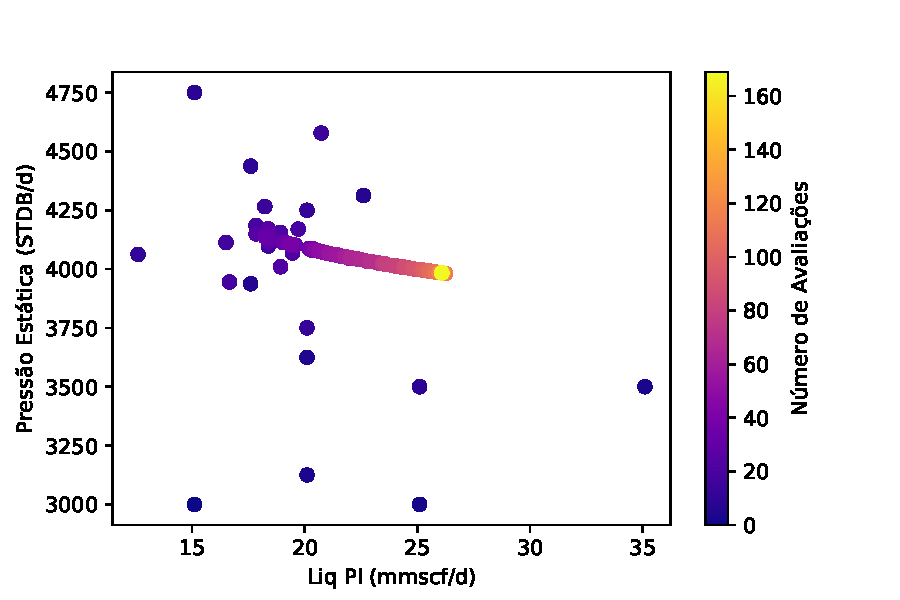
\includegraphics[width=1\linewidth]{figs/setup2_nm_points.pdf}
  \caption{Pontos testados pelo Nelder-Mead.}
  \label{fig:exp2_nm_points}
\end{subfigure}%
\begin{subfigure}{0.5\textwidth}
  \centering
  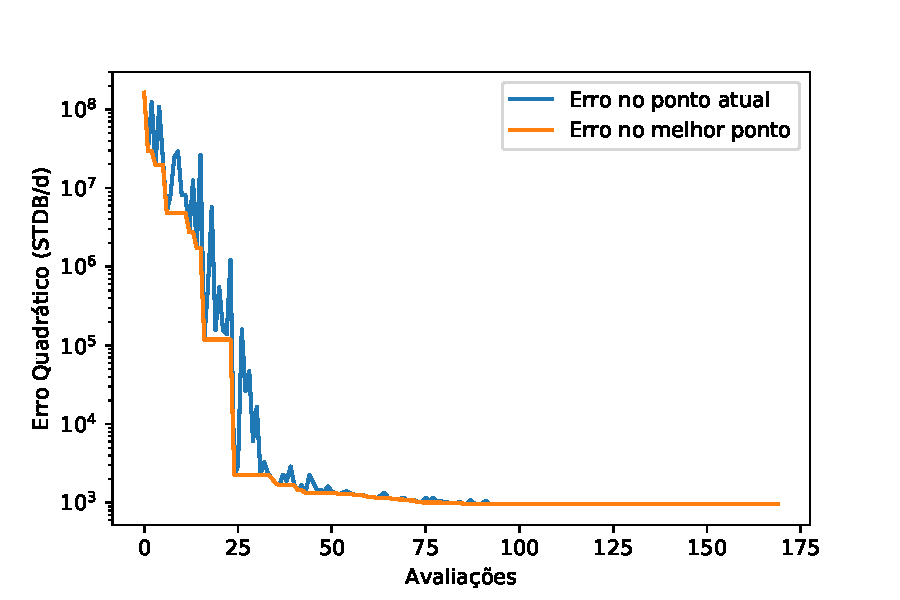
\includegraphics[width=1\linewidth]{figs/setup2_nm_errors.pdf}
  \caption{Erro nos pontos avaliados.}
  \label{fig:exp2_nm_error}
\end{subfigure}
\caption{Nelder-Mead aplicado ao experimento 2.}
\label{fig:exp2_nm}
\end{figure}





\begin{figure}[H]
\centering
  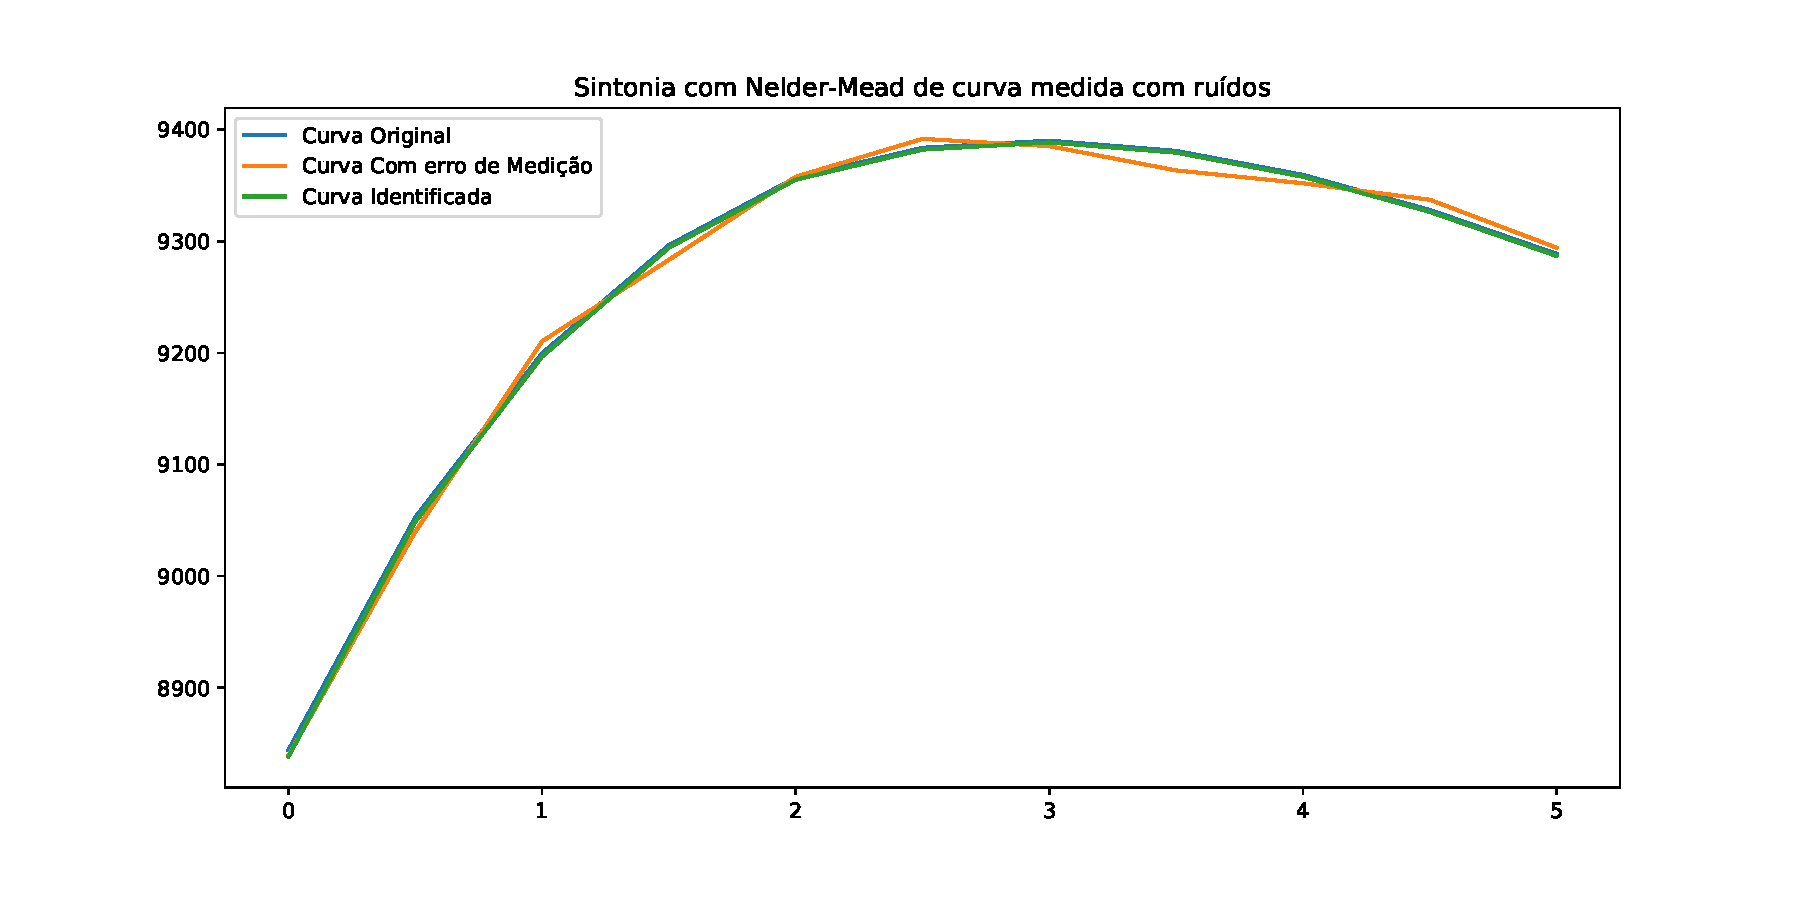
\includegraphics[width=1\linewidth]{figs/curva_nm.pdf}
  \caption{Resultado da sintonia utilizando-se o Nelder-Mead.}
  \label{fig:exp2_nm_curve}
\end{figure}

\section{Discussão}
Nestes experimentos com ruído, não se repete o comportamento anômalo aonde o Nomad com SGTELIB avalia pontos em que aparentemente não há informações relevantes, aumentando sem necessidade o número de iterações e tempo computacional, como pode ser visto na Figura \ref{fig:comp2} e na Tabela \ref{tab:res2}.
%
Pelo contrário, ele acaba sendo o mais eficiente dos três métodos. O Nelder-Mead, por sua vez, tornou-se relativamente mais lento.

%

%

\begin{table}[H]
\centering
\caption{Comparação dos métodos para sintonia de uma curva com ruído de medição}
\label{tab:res2}
\begin{tabular}{|l|l|l|l|}
\hline
                    & Tempo & Iterações & Custo   \\ \hline
OrthoMADS           & 334   & 130       & 956,827 \\ \hline
OrthoMADS + SGTELIB & 187   & 68        & 982,524 \\ \hline
Nelder-Mead         & 217   & 92        & 953,522 \\ \hline
\end{tabular}
\end{table}




\begin{figure}[H]
\centering
  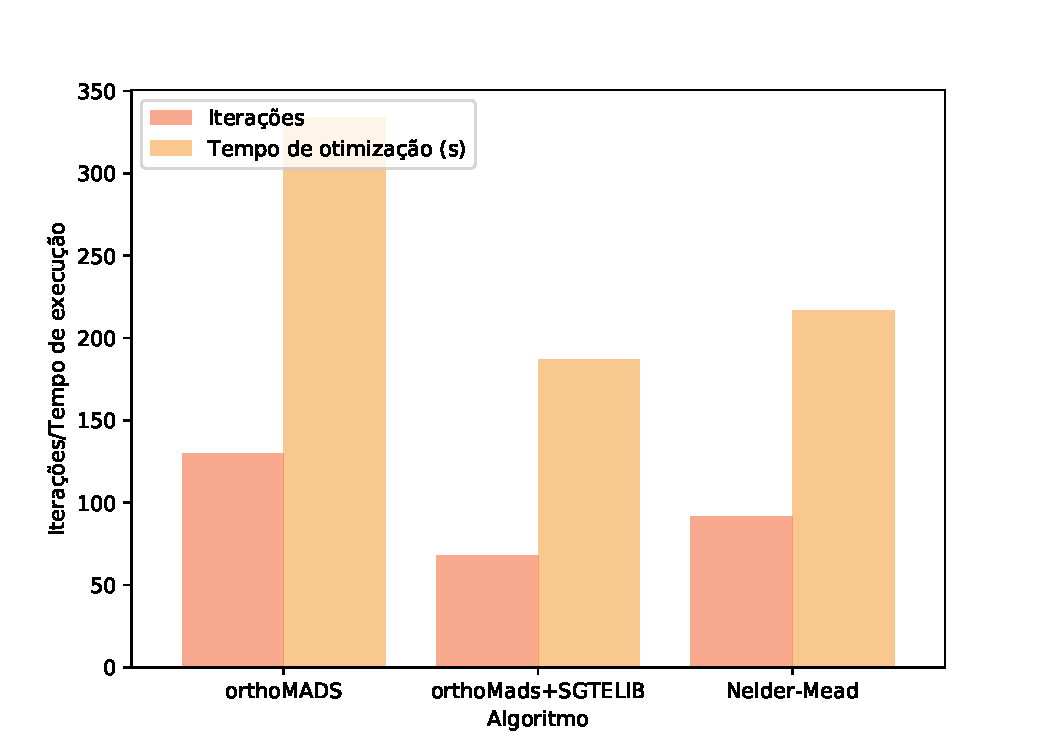
\includegraphics[width=0.7\linewidth]{figs/comp_time_iter_2.pdf}
  \caption{Comparação entre tempos de execução e número de iterações entre os três experimentos com ruído.}
  \label{fig:comp2}
\end{figure}






%%%%%%%%%%%%%%%%%%%
\chapter{Conclusões e Perspectivas}
%
O principal objetivo deste trabalho, que foi utilizar métodos sem derivadas para sintonia de simuladores de escoamento multifásico de óleo e gás, foi alcançado.
%
Foi possível desenvolver e utilizar softwares capazes de interagir com simuladores de fluxo multifásico para, manipulando parâmetros, sintonizar modelos utilizando-se dados experimentais.
%

Desta forma foi mostrado que otimização sem derivadas é uma ferramenta que, dada uma função caixa-preta, é capaz de resolver problemas complexos, encontrando um ponto ótimo em tempo hábil sem necessidade da função explícita ou suas derivadas.
%

Para o futuro, é interessante explorar a opção do pyNOMAD, interface d NOMAD para Python nativa, diminuindo a complexidade envolvida no Opal, e consequentemente simplificando os trabalhos.
%

Outro caminho não explorado é a imposição de restrições adicionais, dependentes do valor da saída do simulador, que podem ser adicionados ao NOMAD para sintonia de redes mais complexas.
%

Além disso, é interessante analisar o Opal, de forma a verificar o motivo do seu uso aparentemente excessivo de poder computacional, além de fazer experimentos com mais núcleos.
%


% ----------------------------------------------------------
% Finaliza a parte no bookmark do PDF
% para que se inicie o bookmark na raiz
% e adiciona espaço de parte no Sumário
% ----------------------------------------------------------
\phantompart

% ---
% Conclusão
% ---
%\chapter{Conclusão}
% ---

% ----------------------------------------------------------
% ELEMENTOS PÓS-TEXTUAIS
% ----------------------------------------------------------
\postextual
% ----------------------------------------------------------

% ----------------------------------------------------------
% Referências bibliográficas
% ----------------------------------------------------------
\bibliography{bibli}{}

% ----------------------------------------------------------
% Glossário
% ----------------------------------------------------------
%
% Consulte o manual da classe abntex2 para orientações sobre o glossário.
%
%\glossary

% ----------------------------------------------------------
% Apêndices
% ----------------------------------------------------------

% ---
% Inicia os apêndices
% ---
\begin{apendicesenv}

% Imprime uma página indicando o início dos apêndices
\partapendices

% ----------------------------------------------------------
\chapter{Revisão de Probabilidade}
\label{appendix:probability}




\end{apendicesenv}
% ---

% ----------------------------------------------------------
% Anexos
% ----------------------------------------------------------

% ---
% Inicia os anexos
% ---
\begin{anexosenv}
\renewcommand\chaptername{Appendix}
% Imprime uma página indicando o início dos anexos
\partanexos
\chapter{Title of Appendix A}
\label{anexo:1}



\end{anexosenv}
%---------------------------------------------------------------------
% INDICE REMISSIVO
%---------------------------------------------------------------------
\phantompart
\printindex
%---------------------------------------------------------------------

\end{document}
